\documentclass[10pt,a4paper]{article}
\usepackage[T1]{fontenc}
\usepackage[english]{babel}
\usepackage{amsmath}
\usepackage{amsfonts}
\usepackage{amssymb}
\usepackage{graphicx}
\usepackage{physics}
\usepackage{bm}
\usepackage{glossaries}
\usepackage[hidelinks]{hyperref}
\usepackage{subcaption}
\usepackage{algorithm}
\usepackage{algpseudocode}
\usepackage{xcolor}
\usepackage{listings}
\usepackage{booktabs}

\lstset{
  language=Python,
  basicstyle=\ttfamily\small,
  keywordstyle=\color{blue!60!black},
  commentstyle=\color{gray},
  stringstyle=\color{green!40!black},
  columns=fullflexible,
  breaklines=true,
  showstringspaces=false,
  frame=single,
  numbers=none,
}



\newacronym{vqe}{VQE}{Variational Quantum Eigensolver}
\newacronym{mcmc}{MCMC}{Markov chain Monte Carlo}
\newacronym{kpo}{KPO}{Kerr-nonlinear parametric oscillators}
\newacronym{cem}{CEM}{Conditional Expectation Matching}
\newacronym{lsb}{LSB}{Langevin Simulated Bifurcation}
\newacronym{srbm}{SRBM}{Semi-Restricted Boltzmann Machine}
\newacronym{tfim}{TFIM}{Transverse Field Ising Model}
\newacronym{qubo}{QUBO}{quadratic unconstrained binary optimization}
\newacronym{sa}{SA}{simulated annealing}
\newacronym{tts}{TTS}{time to solution}
\newacronym{tte}{TTE}{time to $\epsilon$}
\newacronym{rbm}{RBM}{restricted Boltzmann machine}
\newacronym{sr}{SR}{stochastic reconfiguration}
\newacronym{cg}{CG}{conjugate gradient}
\newacronym{jit}{JIT}{just-in-time}
\newacronym{rmse}{RMSE}{root mean squared error}
\newacronym{sapi}{SAPI}{Solver API}

\makeglossaries
\usepackage[left=2cm,right=2cm,top=2cm,bottom=2cm]{geometry}
\author{
Philipp Hanussek\\[0.5em]
\normalsize Master 2 Quantum Information, Sorbonne Universit\'e, Paris, France\\[0.5em]
\normalsize Supervisor: dr hab. Bart{\l}omiej Gardas, IITiS PAN, Gliwice, Poland
}
\title{
\includegraphics[height=1.8cm]{figures/logo/sorbonne-sciences.png}\hspace{2em}
\includegraphics[height=1.8cm]{figures/logo/iitislogo.png}\\[1em]Toward Quantum Competitiveness in Adiabatic Quantum Computing: A Comparative Study of Variational Algorithms}

\begin{document}
\maketitle

\begin{abstract}
We compare classical samplers, quantum annealers, and physics-inspired hardware within a single rigorous framework for quantum-assisted variational Monte Carlo. A restricted Boltzmann machine represents the wavefunction and is trained with stochastic reconfiguration. We evaluate the underlying samplers -- Metropolis, Gibbs, simulated annealing, an FPGA-based solver, and D-Wave quantum annealers (Pegasus, Zephyr) -- on their behavior across different physical models: the transverse-field Ising model and the (frustrated) Heisenberg chain. We assess sampler performance by two metrics under a matched training protocol: time to a validated energy tolerance, and energy consumed to reach it. FPGA is the fastest and most energy-efficient of the metered classical solvers; no QPU energy measurement exists, so no classical-versus-quantum energy comparison is claimed. On time-to-solution, under a $99\%$-confidence-corrected metric that accounts for each solver's occasionally censored seeds, Pegasus(+\gls{cem}) and Zephyr(+\gls{cem}) both scale nearly flat with $N$ and overtake FPGA by the largest system size tested, reversing the near-tie a plain-median reading would suggest; this should not be over-read as established quantum advantage given the small number of system sizes tested and this metric's sensitivity to the convergence criterion's parameters. A native sparse embedding onto the quantum annealer's hardware graph loses representational capacity; embedding multiple problem copies in parallel is a promising direction, but with only three seeds per level and a single converging run at the highest parallelism tested, the data collected here cannot support a quantitative speedup claim. The variational ansatz is restricted to non-negative amplitudes; for the frustrated Heisenberg chain, the Marshall sign rule extends its validity up to moderate frustration.
\end{abstract}

\clearpage

\tableofcontents
\clearpage

\printglossary[type=\acronymtype]
\clearpage

\section{Overview}
Since the development of programmable quantum processors, many claims regarding quantum advantage have been made. Often, these advantage claims did not last long. In this work, we focus exclusively on the D-Wave Quantum Annealer, which leverages quantum technology to solve \gls{qubo} problems. D-Wave is among the first companies to commercially sell quantum computers. In 2025, researchers from D-Wave claimed to have solved a scientifically relevant problem faster using quantum technology than it would have been possible on classical devices~\cite{King_2025}. However, it is currently an open question whether the D-Wave Quantum Annealer is able to solve other problems well, and possibly faster than conventional computers. In this work, we assess D-Wave's ability to sample from a probability distribution, to approximate the ground state of different statistical mechanical models using variational algorithms.  
\subsection{Previous work}
The D-Wave Quantum Annealer's performance scaling for finding the ground state (corresponding to the minimum of the quadratic binary cost function) has been extensively studied, in the area of cryptography and physical simulation. In general, classical methods exhibit faster solving times and better scaling (see \autoref{fig:tta_overview}).

We briefly report on previous work in the field of simulating physical systems using quantum annealing hardware. In \cite{rrf3-jm5m}, we used a method presented in \cite{jalowiecki2020parallel} to encode the solution to the wave function of different Hamiltonians into a \gls{qubo} problem. These instances were then solved on different physical and physics-inspired solvers. We evaluate the scaling of the samplers using the \gls{tts} metric, which corresponds to the computational time needed to solve the optimisation problem with a success probability of at least $P_\text{target}$. The TTS is defined as
\begin{equation}
\text{TTS} = \frac{\ln(1-P_\text{target})}{\ln(1-P_\text{success})} T_r,
\label{eq:tts}
\end{equation}
where $P_\text{success}$ is the probability of obtaining the ground state in a single run, and $T_r$ denotes the runtime of a single run. \autoref{fig:tta-native} shows the resulting TTS for the native, embedding-free formulation of one such Hamiltonian; classical solvers dominate across the entire range tested ($N=16$ to $112$).


Another previous work that we report on is integer factorisation on the D-Wave Annealer, that is, computing the two prime factors $p,q$ of a semiprime $N = p \times q$. \cite{willsch2024state} benchmark three \gls{qubo} adaptations of this problem against uniformly random guessing. \autoref{fig:tta-factoring} reproduces their result: all three encodings still scale exponentially in the number of unknown bits $l = l_p^* + l_q^*$, and only the instances using custom embedding (denoted as CFA\cite{ding2023effectiveprimefactorizationquantum}), asymptotically beats random guessing.

\begin{figure}[htbp]
\centering

\begin{subfigure}{0.48\textwidth}
    \centering
    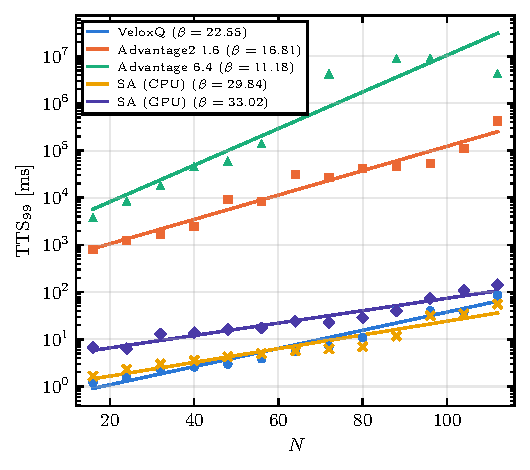
\includegraphics[width=\textwidth]{figures/tta_overview_native.pdf}
    \caption{}
    \label{fig:tta-native}
\end{subfigure}
\hfill
\begin{subfigure}{0.48\textwidth}
    \centering
    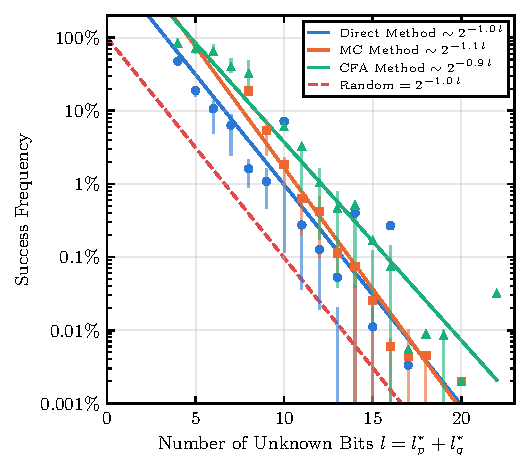
\includegraphics[width=\textwidth]{figures/factoring_success.pdf}
    \caption{}
    \label{fig:tta-factoring}
\end{subfigure}

\caption{Illustration of previous results on solving optimization problems using QPU hardware. \textbf{(a)} TTS99 for simulating a native single-qubit rotation, governed by $H_1 = \frac{\pi}{2}\sigma_y$, vs.\ system size $N$ \cite{rrf3-jm5m}, missing points indicate zero success probability. \textbf{(b)} Success frequency of factoring a semiprime $N = p \times q$ vs.\ the number of unknown bits $l = l_p^* + l_q^*$, reproduced from \cite{willsch2024state}, for three different \gls{qubo} encodings and for uniformly random guessing; markers are the mean success frequency over $\sim\!10$ random semiprimes per $l$, bars span the 25th--75th percentile, and lines are fitted exponential scalings $\propto 2^{-bl}$.}
\label{fig:tta_overview}
\end{figure}

To conclude, results returned by the quantum annealer are inherently noisy. This makes it difficult to sample the \textit{exact} ground state of the submitted Hamiltonian. In this work, we therefore assess the device's ability to act as a Gibbs sampler and sample from the Boltzmann distribution. It has been shown earlier that the D-Wave device can in fact be used as a Gibbs sampler\cite{Mehta_2025,Nelson_2022} and that these samples can be used to train small-scale neural networks to solve many-body problems\cite{Gardas_2018}. In this work we aim to extend the analysis to different many-body models, notably the J1-J2 Heisenberg model, and propose a rigorous comparison between different quantum and classical samplers for bigger system sizes. 
\section{Quantum Models}
\subsection{Quantum Ising Models}
The Ising model consists of discrete spins arranged on a lattice, interacting via nearest-neighbour couplings. In its quantum extension, the \gls{tfim}, a transverse magnetic field is added, introducing quantum fluctuations through non-commuting terms in the Hamiltonian~\cite{mpg}. The Hamiltonian for the one-dimensional \gls{tfim} is given by
\begin{equation}
H=-J\sum_i\sigma_i^z\sigma_{i+1}^z-h\sum_i\sigma_i^x
\label{eq:tfim}
\end{equation}
where $J>0$ is the ferromagnetic coupling strength, $h\geq0$ is the transverse magnetic field strength, and periodic boundary conditions are imposed on the chain. The 1D \gls{tfim} serves as a benchmark for our models, as it is exactly solvable via the Jordan–Wigner transformation. Despite its simplicity, it displays non-trivial quantum behavior, including a quantum phase transition and quantum fluctuations.
\subsection{Heisenberg Models}
The Heisenberg spin chain describes spins on lattice sites interacting via exchange coupling~\cite{Heisenberg_1928}:

\begin{equation}
    H = \sum_{\langle i,j \rangle} J_{ij}\,\boldsymbol{\sigma}_i \cdot \boldsymbol{\sigma}_j
\end{equation}

where $\boldsymbol{\sigma}_i = (\sigma_i^x, \sigma_i^y, \sigma_i^z)$ are the Pauli spin operators, $J_{ij}$ is the exchange coupling between sites $i$ and $j$, and $\langle i,j \rangle$ denotes nearest-neighbour pairs. Spin operators are represented by Pauli matrices (eigenvalues $\pm1$) rather than spin-$\tfrac12$ operators (eigenvalues $\pm\tfrac12$) throughout this work. In contrast to the \gls{tfim}, the Heisenberg model couples all three spin components.

The frustrated $J_1$-$J_2$ Heisenberg chain extends the Heisenberg model with a next-nearest-neighbour exchange term:

\begin{equation}
\label{eq:j1j2heisenberg}
    H = J_1 \sum_{i} \boldsymbol{\sigma}_i \cdot \boldsymbol{\sigma}_{i+1} + J_2 \sum_{i} \boldsymbol{\sigma}_i \cdot \boldsymbol{\sigma}_{i+2},
\end{equation}

where $J_1$ and $J_2$ are the nearest- and next-nearest-neighbour coupling strengths. The competing interactions frustrate the system, preventing simultaneous minimisation of both exchange terms. Setting $J_2 = 0$ recovers the standard Heisenberg chain, while increasing $J_2/J_1$ drives the system into a more frustrated regime that poses a more stringent test for variational methods.
\subsection{Exact Solving}
Determining the exact value of the ground state up to numerical precision is crucial for evaluating the performance of the trained models. For \gls{tfim}, exact solving is possible for arbitrary system sizes, whereas solving the $J_1$-$J_2$ Heisenberg model is computationally hard.
\subsubsection{TFIM ground state solving in \texorpdfstring{$O(N)$}{O(N)}}
The 1D \gls{tfim} defined in \autoref{eq:tfim} can be solved exactly in $O(N)$ time, for $J>0$, $h\geq0$ with periodic boundary condition. We closely follow the method presented in \cite{Lieb1961}\cite{He_2017}, to exactly solve the model, by mapping the spins to fermions using the Jordan-Wigner transformation, and thereby splitting it into a periodic and an antiperiodic boundary-condition sector for the fermions. In accordance with \cite{He_2017}, we find that only the fermionic sector with antiperiodic boundary condition is relevant for analytically computing the ground state. Therefore, using the dispersion relation
\begin{equation}
\omega(k) = \sqrt{J^2+h^2-2Jh\cos(k)}
\end{equation},
the closed form for the ground state is given by
\begin{equation}
E_0 = -\sum_{m=0}^{N-1} \omega\!\left(\frac{\pi(2m+1)}{N}\right),
\qquad
\end{equation}.
We verified this closed-form result numerically against exact diagonalization (\texttt{netket}, using \texttt{scipy}'s sparse \texttt{eigsh}) for $N \in \{4,6,8,10\}$ and $h \in \{0.5, 1.0, 1.5\}$, finding agreement to machine precision ($<10^{-13}$).
\subsubsection{Exact Diagonalization}
In cases where mapping to a quadratic fermion Hamiltonian is not possible, e.g. for the frustrated $J_1$-$J_2$ Heisenberg chain, exact diagonalization is used for small system sizes $N$.
Exact diagonalization works by enumerating all $2^N$ basis states of the Hilbert space, constructing the Hamiltonian as a $2^N \times 2^N$ matrix in that basis, and finding its lowest eigenvalue via the Lanczos algorithm. The Lanczos algorithm avoids diagonalizing the entire matrix and only returns the matrix's lowest eigenvalue. We use \texttt{scipy}'s \texttt{eigsh} implementation of this algorithm.
\section{Classical and quantum samplers}
\subsection{Adiabatic Quantum Computing}
\label{sec:solvers:quantum:adiab}
 Adiabatic Quantum Computing is based on the adiabatic theorem, which states: \textit{A physical system remains in its instantaneous eigenstate if a given perturbation is acting on it slowly enough and if there is a gap between the eigenvalue and the rest of the Hamiltonian's spectrum.}
In this work we focus on the D-Wave Quantum Annealer, which acts according to the adiabatic theorem in the following way: 
In the beginning of the annealing process, the device is initiated in the ground state of an initial driver Hamiltonian $H_D$ that can be easily constructed:
\begin{equation}
H_D=-\sum_{i=1}^N \sigma_x^{(i)} \text{ with ground state } \ket{+}^{\otimes N}
\end{equation}
where $\sigma_x$ and $\sigma_z$ are the Pauli matrices acting on qubit $i$. The problem Hamiltonian is defined as
\begin{equation}
H_P=\sum_{i=1}^N h_i\sigma_z^{(i)}+\sum_{i=1}^N\sum_{j=1}^{i-1} J_{ij}\sigma_z^{(i)}\otimes\sigma_z^{(j)}.
\end{equation}
During the annealing process, the system is slowly brought from $H_D$ to $H_P$
according to the so-called annealing schedules $A(s)$ and $B(s)$:
\begin{equation}
H(s) = A(s)H_D + B(s)H_P
= -A(s)\sum_{i=1}^{N} \sigma_x^{(i)}
+ B(s)\sum_{i=1}^{N} h_i \sigma_z^{(i)}
+ B(s)\sum_{i=1}^{N}\sum_{j=1}^{i-1} J_{ij}\, \sigma_z^{(i)} \otimes \sigma_z^{(j)},
\label{eq:annealing_hamiltonian}
\end{equation}
where $s \in [0,1]$ is the normalized time. $A(s)$ decreases the driving terms in $H_D$ as $s$ increases,
and $B(s)$ activates the terms of the problem Hamiltonian $H_P$. At the end of the evolution, if the process happens slow enough, and assuming a noiseless environment, the system will be in the ground state of the problem Hamiltonian according to the adiabatic theorem.
It is important to note that the qubits in the D-Wave Quantum Annealer are not \textit{all-to-all} connected. The qubits are arranged in an architecture dependent grid. In the Pegasus topology, one qubit couples on average to 15 other qubits, while Zephyr qubits couple on average to 20 other qubits. Therefore, most problems require an additional embedding step, in which multiple physical qubits are \textit{chained} together to form one logical qubit. For a toy-problem example of embedding a triangle shaped connectivity pattern on a QPU, see \autoref{fig:embedding-toy-result}. As all problems examined in this work can be represented as bipartite graphs, we use \texttt{minorminor.busclique}, which is part of D-Wave's Ocean SDK.
\begin{figure}[htbp]
    \centering
    \begin{subfigure}[]{0.30\linewidth}
        \centering
        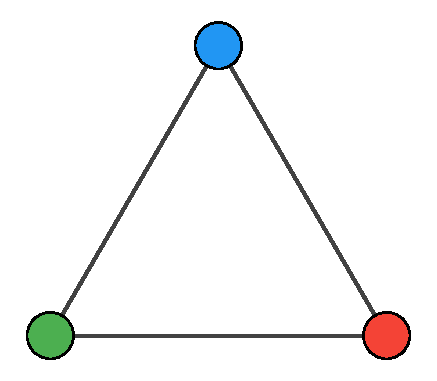
\includegraphics[width=\linewidth]{figures/embedding/a.pdf}
        \caption{}
        \label{fig:embedding-toy-source}
    \end{subfigure}
    \hfill
    \begin{subfigure}[]{0.30\linewidth}
        \centering
        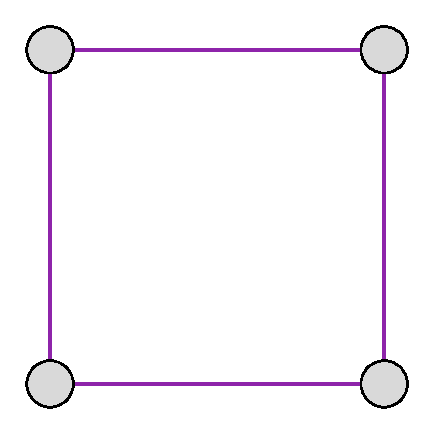
\includegraphics[width=\linewidth]{figures/embedding/b.pdf}
        \caption{}
        \label{fig:embedding-toy-target}
    \end{subfigure}
    \hfill
    \begin{subfigure}[]{0.30\linewidth}
        \centering
        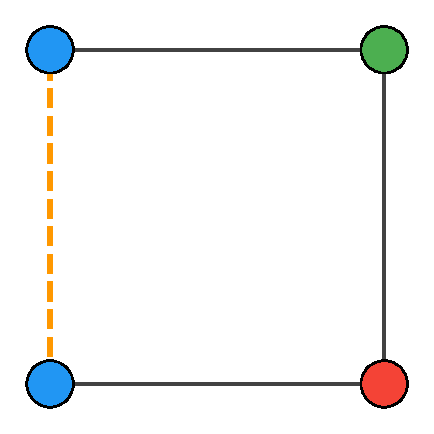
\includegraphics[width=\linewidth]{figures/embedding/c.pdf}
        \caption{}
        \label{fig:embedding-toy-result}
    \end{subfigure}

    \vspace{0.5em}
    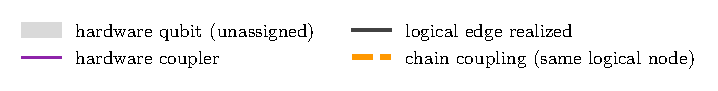
\includegraphics[width=0.7\linewidth]{figures/embedding/legend.pdf}

    \caption{Minor embedding of a triangle onto a sparser hardware graph.\textbf{(a)} Logical problem graph: a triangle requires a coupler between every pair of nodes. \textbf{(b)} Target hardware graph: a 4-cycle, whose qubits admit no triangle directly. \textbf{(c)} A valid embedding: one logical node is realized as a chain of two physical qubits (joined by a strong ferromagnetic coupling, dashed), so that the three logical edges are each realized by a single physical coupler.}
    \label{fig:embedding-toy}
\end{figure}
There exist three different types of couplers, connecting physical qubits: 
\begin{itemize}
\item \textbf{Internal Couplers} connecting qubits of opposite orientation
\item \textbf{External Couplers} connecting qubits aligned in parallel
\item \textbf{Odd Couplers} which connect similarly aligned pairs of qubits
\end{itemize}
\begin{figure*}[ht]
\subfloat[\label{fig:anneal-schedule}]{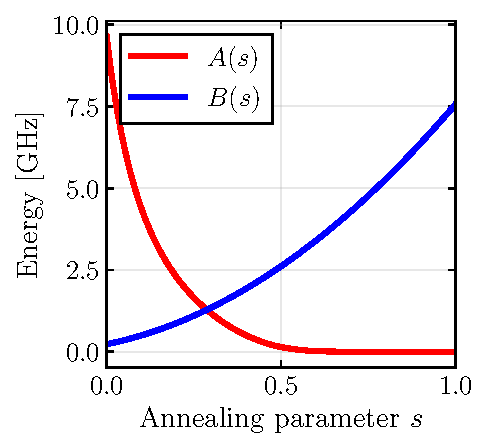
\includegraphics[width=0.33\linewidth]{figures/anneal_schedule_plot.pdf}}%
    \subfloat[\label{fig:anneal-pegasus}]{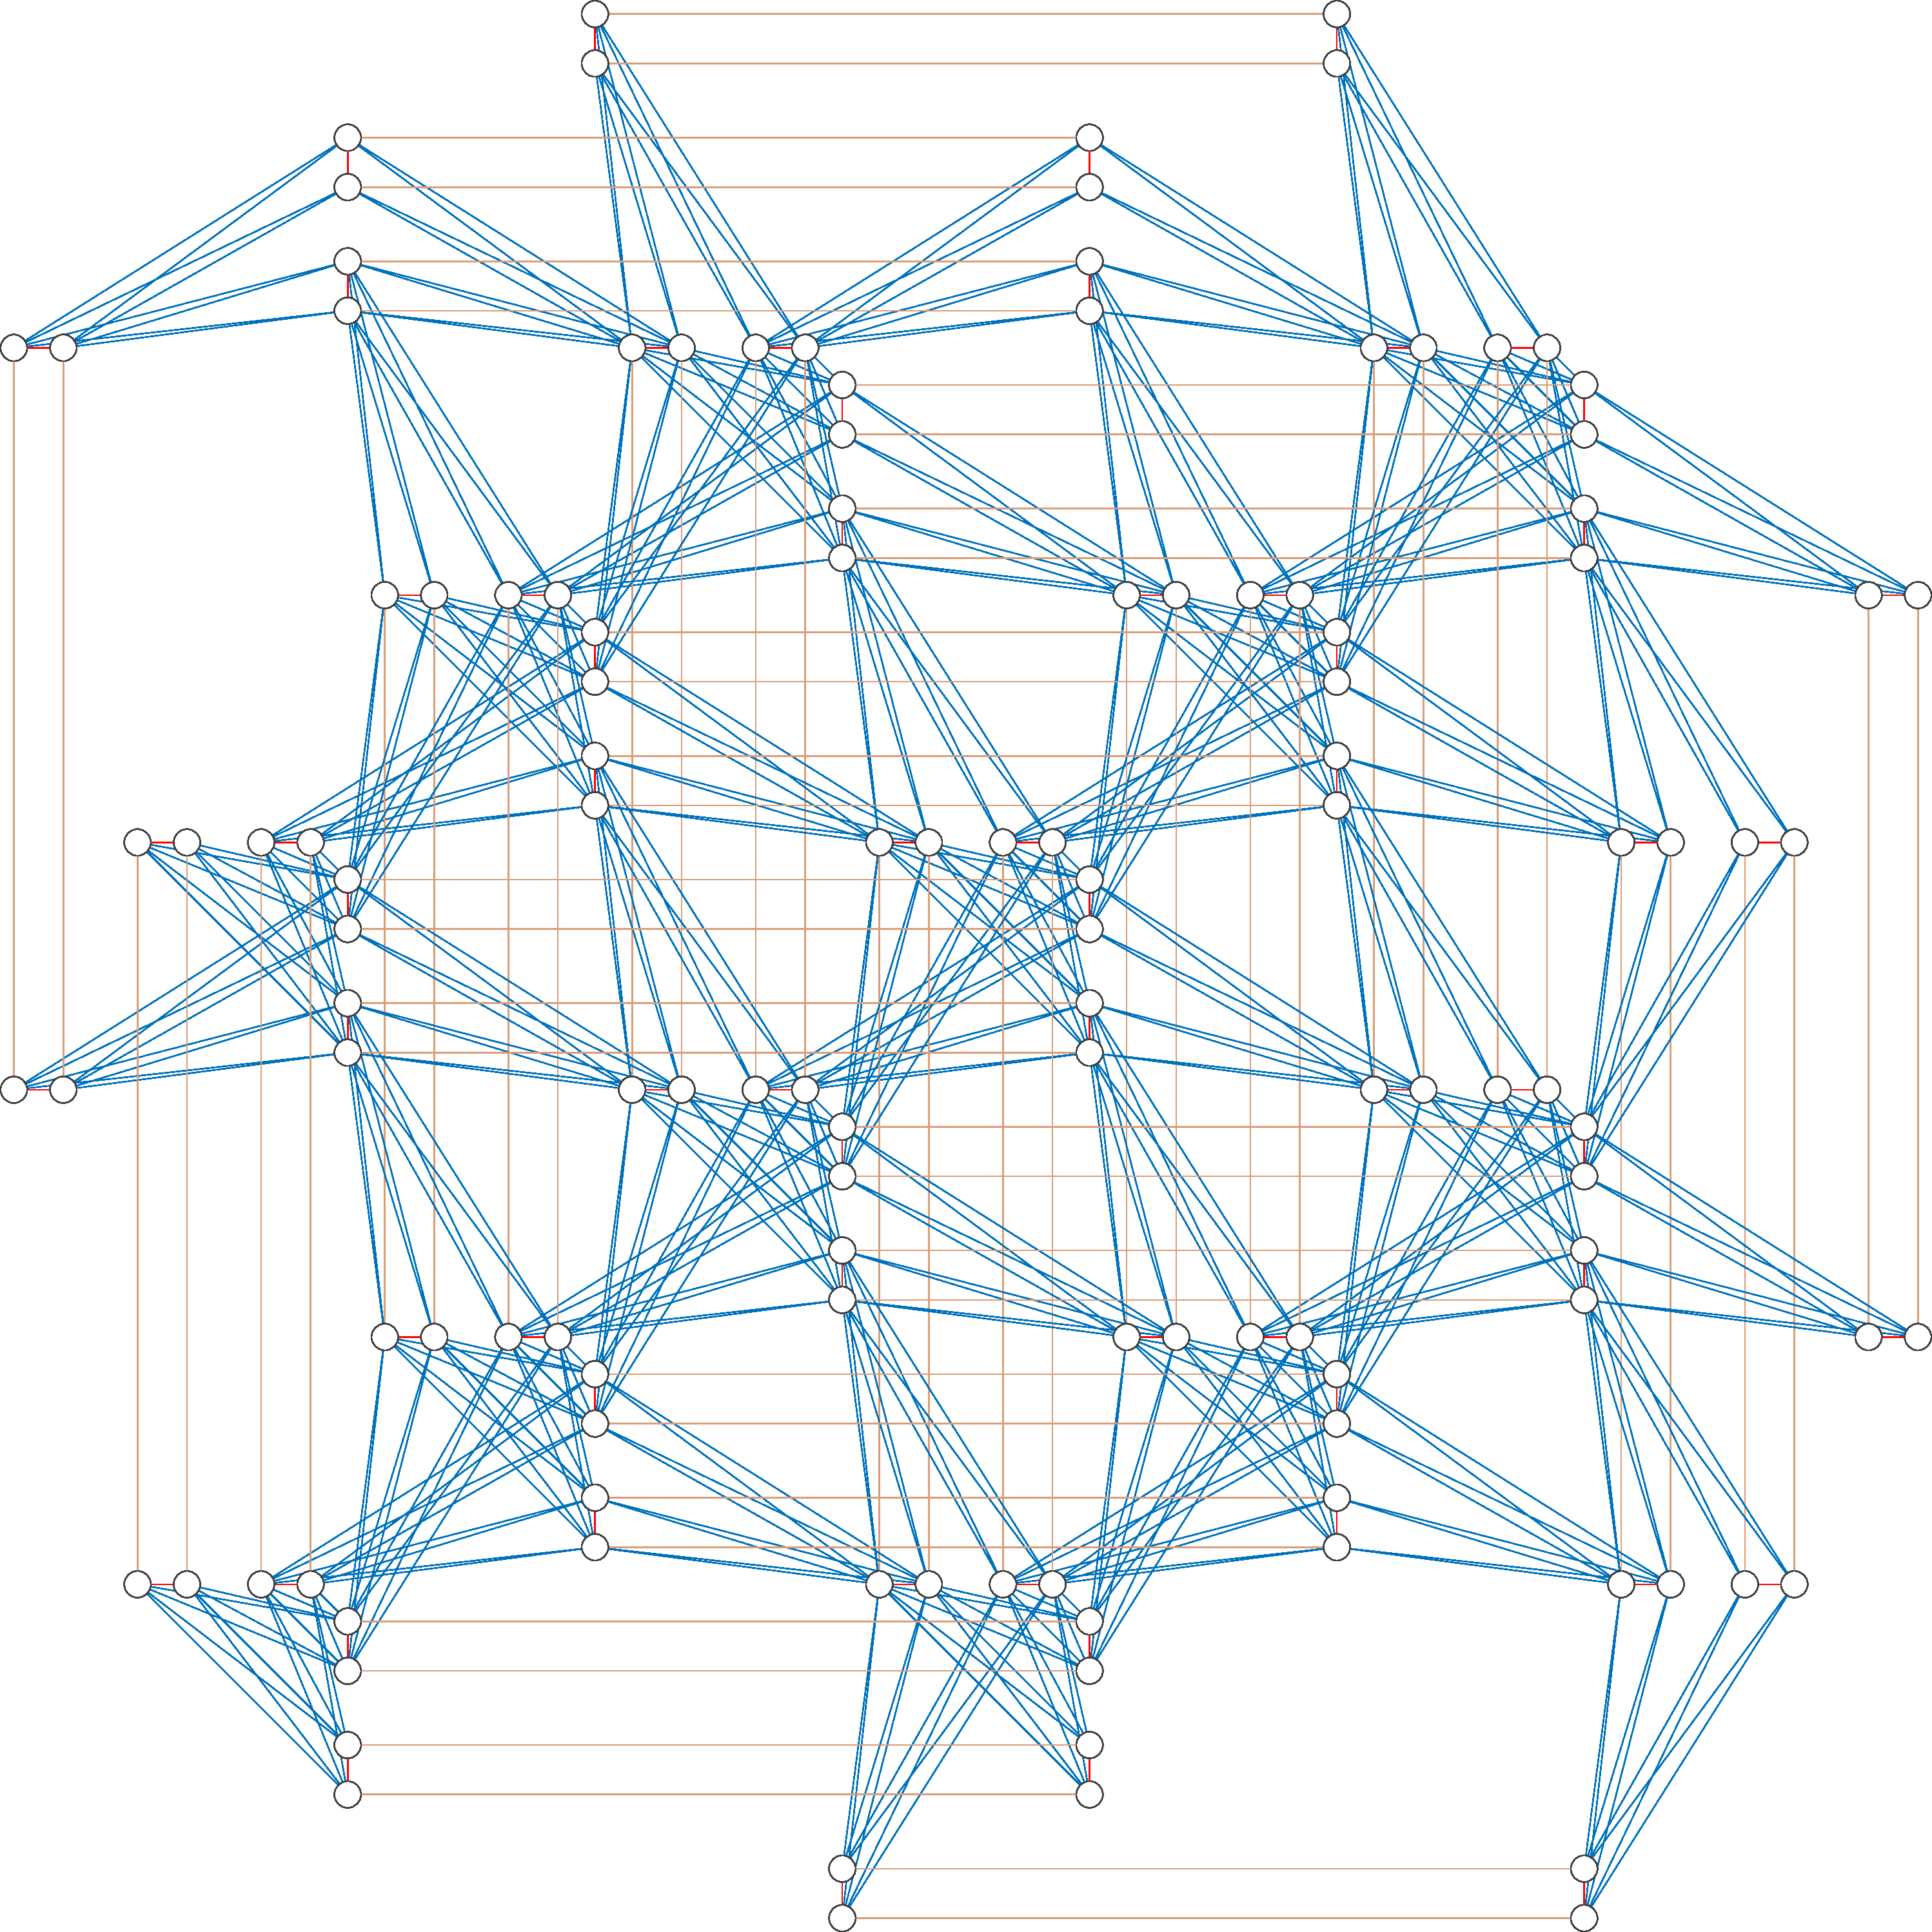
\includegraphics[width=0.33\linewidth]{figures/pegasus.pdf}}%
    \subfloat[\label{fig:anneal-zephyr}]{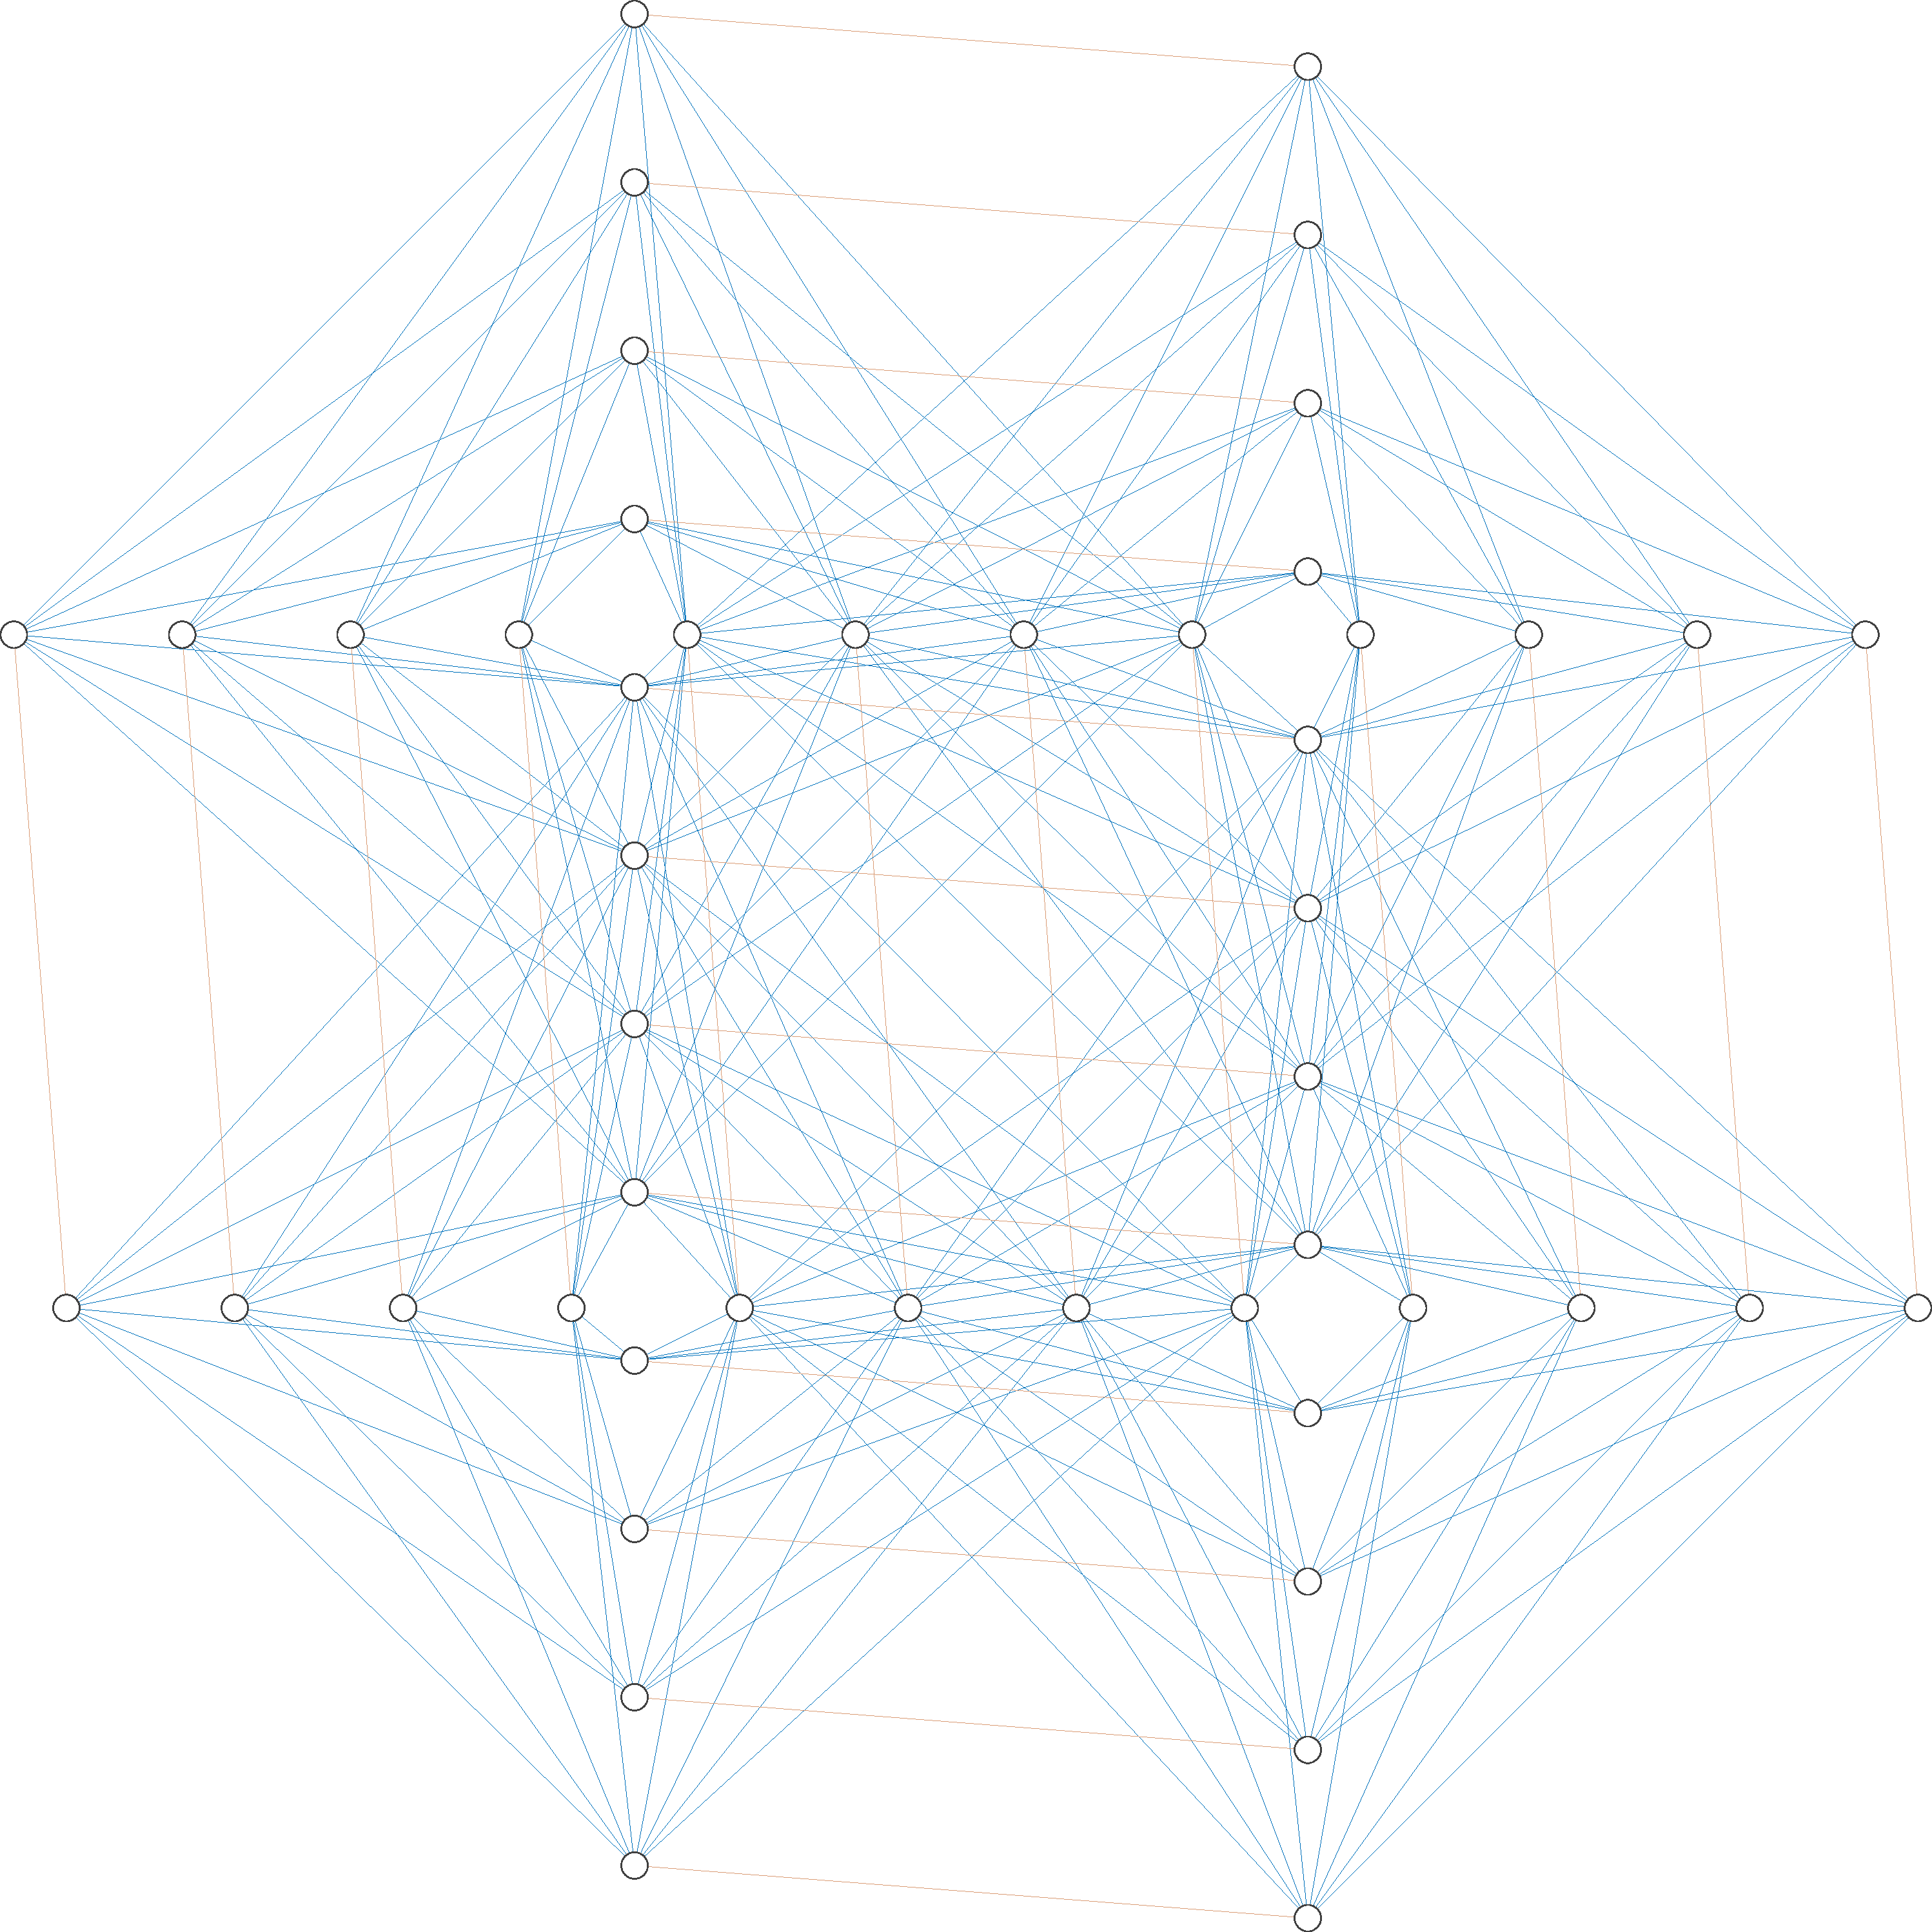
\includegraphics[width=0.33\linewidth]{figures/zephyr.pdf}}
\caption{(a) Time-dependent energy scales executed by the D-Wave quantum annealer. The coefficient $A(s)$ (red) multiplies the transverse-field term that enables quantum tunnelling and therefore falls rapidly as the run progresses. The coefficient $B(s)$ (blue) multiplies the problem Hamiltonian and rises smoothly, so that the device moves from a tunnelling-dominated regime at $s=0$ to a problem-dominated regime at $s=1$. (b) Native connectivity map for the Pegasus architecture (D-Wave Advantage). Circles mark individual superconducting qubits; blue lines are internal couplers and orange lines mark external couplers (c) Connectivity map for the newer Zephyr architecture (D-Wave Advantage2), which increases the number of couplers per qubit and introduces longer-range links.}
\label{fig:anneal:overview}
\end{figure*}
See \autoref{fig:anneal:overview} for visualization of different QPU topologies. 
\subsection{Metropolis-Hastings inspired methods}
We use several \gls{mcmc} methods to generate samples from probability distribution from which direct sampling would be difficult. All of these methods can be traced back to the Metropolis-Hastings algorithm~\cite{Metropolis_1953,Hastings_1970}, which we explain below.
\subsubsection{Metropolis-Hastings Algorithm}
The Metropolis-Hastings Algorithm is a \gls{mcmc} method used to obtain samples from a (multivariate) probability distribution $P(x)$ from which sampling is difficult. The goal of the algorithm is to define a Markov chain whose stationary distribution is $P(x)$. Suppose we can evaluate an unnormalized target density $f(x)$, where $f(x) \propto P(x)$, and the normalization constant is unknown. In the \textbf{proposal} step, a \textit{candidate} $x^*$ from a proposal distribution $q(x^*| x_n)$ is generated, $x_n$ being the current state of the Markov chain. In the \textbf{accept-reject} step, the acceptance probability $A(x_n\rightarrow x^*)$ is calculated\cite{djnavarroMetropolisHastingsAlgorithm}:
\begin{equation}
A(x_n\rightarrow x^*) =\min\left(1, \frac{f(x^*)}{f(x_n)}\times\frac{q(x_n|x^*)}{q(x^*|x_n)}\right).
\end{equation}
For the evaluation of $\frac{f(x^*)}{f(x_n)}$, knowledge of the normalization constant is not necessary. The candidate $x^*$ is accepted with probability $A(x_n\rightarrow x^*)$.
\subsubsection{Simulated Annealing}
\Gls{sa}~\cite{Kirkpatrick_1983} is the classical analogue and predecessor of quantum annealing. It works by exploring the neighborhood of a given configuration, accepting the proposed solution with a temperature dependent probability, or if the new configuration has a lower energy than the current one. In this work, we use a geometrical temperature schedule\cite{YANG201467} instead of a linear one. The schedule is given by the formula
\begin{equation}
T_k = T_{\text{initial}}\left(\frac{T_{\text{final}}}{T_{\text{initial}}}\right)^{k/(n_{\text{steps}}-1)},\qquad k = 0, 1, \dots, n_{\text{steps}}-1,
\end{equation}
where $T_{\text{initial}}$ and $T_{\text{final}}$ are the starting and target temperatures and $n_{\text{steps}}$ is the total number of annealing steps.

\subsection{Gibbs Sampling}
\label{sec:gibbs}
Gibbs sampling~\cite{Geman_1984} is used when sampling directly from a joint distribution is difficult, but sampling from the full conditional distributions is tractable. The algorithm constructs a Markov chain by iteratively sampling each variable (or block of variables) from its distribution conditioned on the current values of all other variables. This procedure generates a chain whose stationary distribution is the target joint distribution. In this work we use an adapted version of this procedure, \textit{blocked} Gibbs sampling, which allows to sample from all the hidden (visible) variables together. We closely follow the method description given in D'Angelo et al.\cite{PhysRevResearch.2.023266}. As we are using a \gls{rbm} which by definition is bipartite without any intra-layer connections, there is  mutual independence between the hidden (visible) variables if the visible (hidden) variables are held fixed. The blocked Gibbs sampling can then be described by the following equations:

\begin{equation}
  p(h_j = +1 \mid \mathbf{v}) = \sigma\!\left(2\left(b_j + \sum_{i} W_{ij}
  v_i\right)\right), \qquad
  p(v_i = +1 \mid \mathbf{h}) = \sigma\!\left(2\left(\sum_{j} W_{ij} h_j -
  a_i\right)\right),
\end{equation}
with $\sigma(x) = 1/(1+e^{-x})$, $\mathbf{a}$ the visible bias, $\mathbf{b}$ the hidden bias, and $W$ the weight matrix. Since $h_j, v_i \in \{-1,+1\}$, each unit is sampled by drawing $u \sim \mathcal{U}(0,1)$ and setting the unit to $+1$ if $u < p(\cdot=+1\mid\cdot)$, else $-1$.                                          
One full block-Gibbs sweep is                                                                      
\begin{equation}
  \mathbf{h} \sim p(\mathbf{h}\mid\mathbf{v}), \qquad \mathbf{v}' \sim
  p(\mathbf{v}\mid\mathbf{h}),
\end{equation}                                                                                                                                         
with all components of $\mathbf{h}$ (resp. $\mathbf{v}'$) drawn simultaneously. Before sampling for the first time, we initialize the sampler by performing a so-called \textit{warm-up}, that is, performing 200 full block-Gibbs sweeps to allow the chain to converge to its stationary distribution (in the optimal case). Under the \textit{persistent chain} assumption from \cite{PhysRevResearch.2.023266}, no warm-up is performed for subsequent sampling calls. The PCD assumption states that the chain stays near-equilibrium for small parameter changes.
\section{Variational Algorithms}
Variational algorithms are a class of hybrid quantum-classical optimization methods designed to find the ground state of a given Hamiltonian. Unlike the \acrfull{vqe}, which prepares and measures a parametrised circuit on a gate-based quantum computer, this work uses quantum-assisted Variational Monte Carlo: a classical neural-network ansatz~\cite{Carleo_2017} is optimised via Stochastic Reconfiguration, and a quantum device is used only to generate samples of that ansatz. Variational Monte Carlo consists of three parts: the \textit{cost function} to be minimized, the \textit{ansatz}, which in our case is a Boltzmann machine, and an \textit{expectation value estimation}. Additionally, a classical optimizer is needed to improve the ansatz at each iteration. Depending on how the ansatz is realised on quantum hardware, two approaches for estimating the expectation value are possible:
\begin{itemize}
	\item On gate-based quantum computers, measuring can be used to gather expectation values of the modified ansatz and improve it further
	\item In adiabatic quantum computing, the quantum device is used to generate representative samples of the modified ansatz. These samples are then used to approximate the expectation value. 
\end{itemize}
As we are interested in comparing current quantum annealing devices with their classical counterparts, we focus solely on the second case. 
\subsection{Restricted Boltzmann Machine}
Different constructions for the ansatz are possible, here we focus on a \gls{rbm} which has been shown to successfully approach the ground state in previous  works\cite{PhysRevResearch.2.023266,Carleo_2017,Gardas_2018}. A \gls{rbm} is an artificial neural network consisting of visible and hidden units that form a bipartite graph, without intra-layer connections. It has been shown to be a universal approximator, meaning that it can represent any desired probability distribution to arbitrary accuracy\cite{10.1162/neco.2008.04-07-510}, give a sufficient number of hidden units. The main idea is that expectation values with respect to the quantum state can be estimated using samples drawn from the probability distribution $|\Psi(\mathbf{v})|^2$. Since the wavefunction ansatz is represented by a Restricted Boltzmann Machine, which corresponds to a classical stochastic Ising model, configurations $\mathbf{v}$ can be sampled approximately using a D-Wave quantum annealer.
Commonly for \glspl{rbm}, the ansatz is defined via an energy function over visible and hidden units,
\begin{equation}
E_{\boldsymbol\theta}(\mathbf{v},\mathbf{h})=\mathbf{a}\cdot \mathbf{v} -\mathbf{b}\cdot \mathbf{h} - \mathbf{h}\cdot \mathbf{W}^\top \cdot \mathbf{v},
\end{equation}
with weights $\boldsymbol\theta=\{\mathbf{a}, \mathbf{b}, \mathbf{W}\}$ respectively applied to the vector of visible units $\mathbf{v}=(v_1, \ldots, v_N)\in\{-1,+1\}^N$ and hidden units $\mathbf{h}=(h_1, \ldots, h_M)\in\{-1,+1\}^M$. Throughout, $\mathbf{W}\in\mathbb{R}^{N\times M}$ is indexed visible-by-hidden, $W_{ij}$ with $i$ the visible and $j$ the hidden index, matching its representation in the implementation. The joint quantum state is
\begin{equation}
\label{eq:rawansatz}
\ket\Psi =\sum_{\mathbf{v}}\Psi(\mathbf{v})\ket{\mathbf{v}}, \qquad \Psi(\mathbf{v})=\sqrt{\sum_{\mathbf{h}} e^{-E_{\boldsymbol\theta}(\mathbf{v},\mathbf{h})}},
\end{equation}
so that $|\Psi(\mathbf{v})|^2=\sum_{\mathbf{h}} e^{-E_{\boldsymbol\theta}(\mathbf{v},\mathbf{h})}$ is, up to normalization, the marginal over hidden units of the joint Boltzmann distribution $p_{\boldsymbol\theta}(\mathbf{v},\mathbf{h})=Z^{-1}e^{-E_{\boldsymbol\theta}(\mathbf{v},\mathbf{h})}$, $Z=\sum_{\mathbf{v},\mathbf{h}}e^{-E_{\boldsymbol\theta}(\mathbf{v},\mathbf{h})}$, i.e.\ $|\Psi(\mathbf{v})|^2 \propto \sum_{\mathbf{h}} p_{\boldsymbol\theta}(\mathbf{v},\mathbf{h})$. The corresponding Born probability distribution is
\begin{equation}
\rho(\mathbf{v})=\frac{|\Psi(\mathbf{v})|^2}{\sum_{\mathbf{v}'}|\Psi(\mathbf{v}')|^2},
\end{equation}
which is however intractable to normalize for large Hilbert spaces.
Tracing out the hidden variables in \autoref{eq:rawansatz}, the ansatz becomes\cite{Carleo_2017}:
\begin{equation}
\label{eq:ansatz}
\Psi(\mathbf{v}) = e^{-\mathbf{a} \cdot \mathbf{v}/2} \prod_{j=1}^{N_h} \left[ 2\cosh\!\left(b_j + \sum_i W_{ij} v_i\right) \right]^{1/2}.
\end{equation}
Two sampling regimes are used in this work. Classical Metropolis-Hastings samples directly from the closed-form marginal $\Psi(\mathbf{v})$ of \autoref{eq:ansatz}: only the visible units are instantiated, and $\mathbf{h}$ never appears as an explicit random variable. Gibbs sampling on the D-Wave annealer instead targets the joint distribution $p_{\boldsymbol\theta}(\mathbf{v},\mathbf{h})$: both $\mathbf{v}$ and $\mathbf{h}$ are encoded as physical qubits (\autoref{fig:rbm-embedding}), the annealer returns samples of the pair $(\mathbf{v},\mathbf{h})$. $\mathbf{h}$ is subsequently marginalized to obtain samples of $\mathbf{v}$ distributed as $\rho(\mathbf{v})$.
\subsection{Training a RBM}
The \gls{rbm} training loop can be summarized in four steps:
\begin{enumerate}
\item Sampling a configuration of visible variables $\mathbf{v}$ using classical / QPU samplers (see previous section)
\item Calculating the \textbf{local energies}: The local energy is given by
\begin{equation}
E_\text{loc}(\mathbf v)=\frac{\langle \mathbf v|H|\Psi\rangle}{\Psi(\mathbf v)}
\end{equation}
(see \autoref{eq:localenergy} for the expanded form used during training). For the \gls{tfim} \eqref{eq:tfim}, evaluating this only requires the ansatz \eqref{eq:ansatz} at the current configuration and at each single-spin-flipped configuration $\bar{\mathbf v}_i$ (i.e.\ $\mathbf v$ with $v_i \to -v_i$)\cite{Gardas_2018,Carleo_2017}:
\begin{equation}
E_\text{loc}(\mathbf v) = -J\sum_{\langle i,j\rangle} v_i v_j - h\sum_i \frac{\Psi(\bar{\mathbf v}_i)}{\Psi(\mathbf v)}.
\end{equation}
For the Heisenberg and frustrated $J_1$-$J_2$ chains \eqref{eq:j1j2heisenberg}, the off-diagonal part works differently\cite{Carleo_2017,Sorella_1998}. Instead of a field flipping one spin at a time, the $\sigma^x_i\sigma^x_j+\sigma^y_i\sigma^y_j$ exchange term flips a \emph{pair} of spins $(i,j)$ together, and only when they point in opposite directions ($v_i\neq v_j$): flipping two equal spins would just reproduce $\mathbf v$ itself, so that term contributes nothing. Writing $\bar{\mathbf v}_{ij}$ for $\mathbf v$ with both $v_i$ and $v_j$ flipped, and $s\in\{-1,+1\}$ for the Marshall sign (\autoref{sec:marshall}, applied only to nearest-neighbour bonds), the local energy is
\begin{equation}
E_\text{loc}(\mathbf v) = J_1\sum_i v_iv_{i+1} + J_2\sum_i v_iv_{i+2}
 + 2J_1 s\!\!\sum_{i:\,v_i\neq v_{i+1}}\!\!\frac{\Psi(\bar{\mathbf v}_{i,i+1})}{\Psi(\mathbf v)}
 + 2J_2\!\!\sum_{i:\,v_i\neq v_{i+2}}\!\!\frac{\Psi(\bar{\mathbf v}_{i,i+2})}{\Psi(\mathbf v)}.
\end{equation}
The local energy formulation given here is an extension of the version given in Carleo et al.\cite{Carleo_2017}, as it includes the additional terms to take into account the next-nearest-neighbour $J_2$ coupling\cite{Sorella_1998}. In this work, the \gls{rbm} is restricted to be real-valued (in contrast to the complex-valued \gls{rbm} used in \cite{Carleo_2017}). Consequently, we need to apply a sign correction $s$ to the $J_1$ term.

\item Calculating the \textbf{log-derivatives}: Since the ansatz \eqref{eq:ansatz} already has the hidden units traced out, the gradient observable $O_k$ needed for \gls{sr} (\autoref{sec:stochsticreconfig}) can likewise be evaluated from the visible units alone. Writing $\theta_j = b_j + \sum_i W_{ij} v_i$,
\begin{equation}
\frac{\partial \log \Psi(\mathbf v)}{\partial \theta_k} = \frac{1}{2}
\begin{cases}
-v_i, & \theta_k = a_i\\
\tanh(\theta_j), & \theta_k = b_j\\
v_i \tanh(\theta_j), & \theta_k = W_{ij}.
\end{cases}
\end{equation}
\item Updating the \textbf{parameters} $\boldsymbol\theta=\{\mathbf a,\mathbf b,\mathbf W\}$ via \gls{sr}, as detailed in \autoref{sec:stochsticreconfig}.
\end{enumerate}
\begin{figure}[htbp]
    \centering
    \begin{subfigure}{0.6\linewidth}
        \centering
        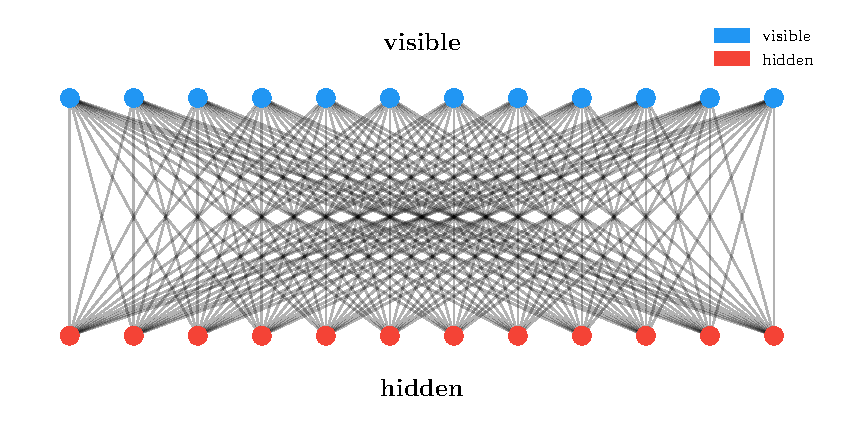
\includegraphics[width=\linewidth]{figures/rbm_abstract.pdf}
        \caption{}
        \label{fig:rbm-abstract}
    \end{subfigure}
    \hfill
    \begin{subfigure}{0.3\linewidth}
        \centering
        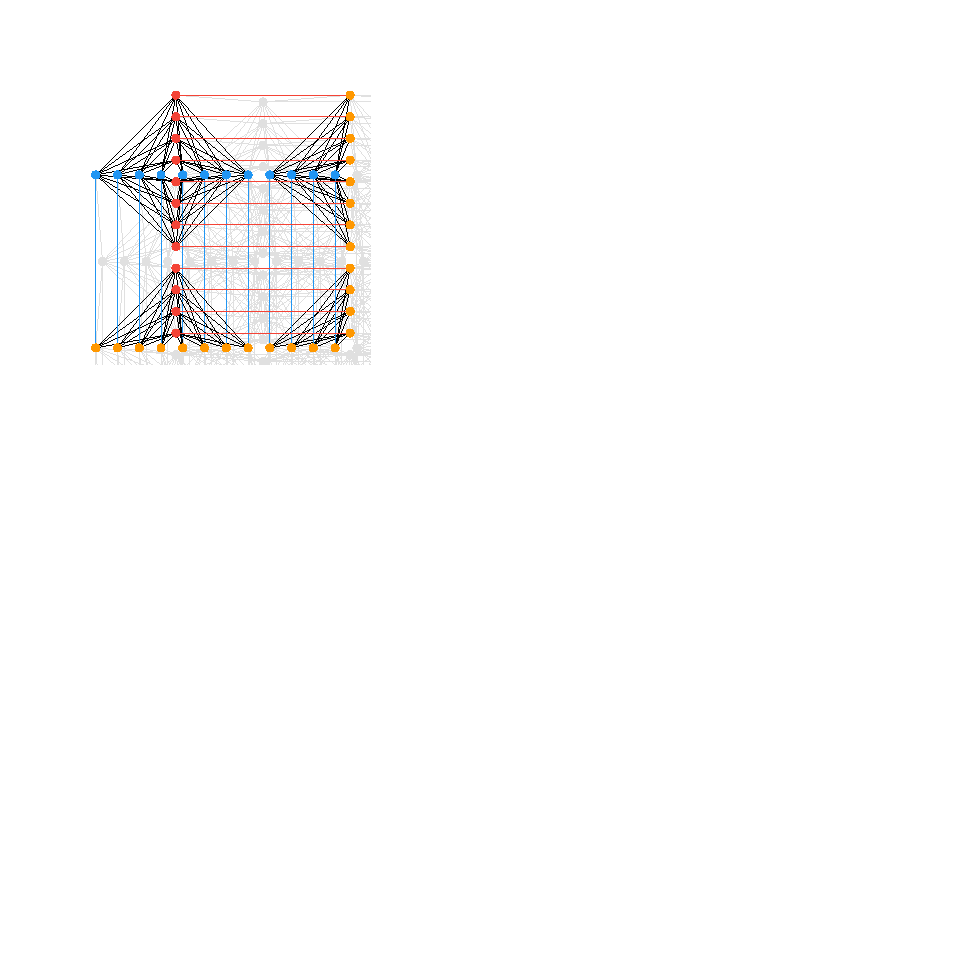
\includegraphics[width=\linewidth]{figures/embedding_full_zephyr.pdf}
        \caption{}
        \label{fig:embedding-zephyr}
    \end{subfigure}
    \caption{(a) RBM with $12$ visible and $12$ hidden units. (b) Embedding of the corresponding bipartite graph onto the Zephyr hardware topology. Blue nodes are visible units, red nodes are hidden units, orange nodes are auxiliary chain qubits. Each physical node is connected to one auxiliary qubit.}
    \label{fig:rbm-embedding}
\end{figure}
\subsection{Stochastic gradient descent versus Stochastic reconfiguration}
\label{sec:stochsticreconfig}
Traditionally, neural networks are trained using gradient descent. We will not go into details about this well known approach, as it is extensively covered by literature. Gradients are computed efficiently using backpropagation which exploits the chain rule, reusing intermediate derivatives to evaluate the compositions of continuous functions. Carleo et al., in their article on using neural networks for solving many-body problems (\cite{Carleo_2017}) instead use a method known as Stochastic Reconfiguration, first described by Sorello et al. in \cite{Sorella_1998,Sorella_2001}. The main advantage of \gls{sr} over gradient descent is that it exploits more knowledge about the ansatz than gradient descent. In particular, gradient descent lives in the \textit{parameter space}, and does not take into account the influence of parameter changes on the actual wave function \textit{probability space} $|\Psi|^2$.

\subsubsection{Stochastic reconfiguration}
\gls{sr} is implemented as follows: given the logarithmic derivative for each parameter $k$, that is the gradient observable
\begin{equation}
    O_k(\mathbf{v}) = \frac{\partial \log \Psi(\mathbf{v})}{\partial \theta_k},
\end{equation}
with $\boldsymbol{\theta} = \{\mathbf{a}, \mathbf{b}, \mathbf{W}\}$, the energy gradient or force vector is defined as
\begin{equation}
    F_k = \langle O_k E_\text{loc} \rangle - \langle O_k \rangle \langle E_\text{loc} \rangle,
\end{equation}
which is the covariance of the gradient observable and the local energy. The local energy $E_\text{loc}(\mathbf{v})$ estimates the variational energy $\langle H \rangle$ of the current \gls{rbm} ansatz using samples drawn from $|\Psi(\mathbf{v})|^2$\cite{Carleo_2017}:
\begin{equation}
\label{eq:localenergy}
  E_\text{loc}(\mathbf{v}) = \frac{\langle \mathbf{v} | H | \Psi \rangle}{\langle
  \mathbf{v} | \Psi \rangle} = \sum_{\mathbf{v}'} H_{\mathbf{v}\mathbf{v}'}
  \frac{\Psi(\mathbf{v}')}{\Psi(\mathbf{v})}
\end{equation}



The next step then is to define the quantum geometric tensor $\mathbf{S}$, the regularised sample covariance of the $O_k$ vectors, which measures how sensitive the Born distribution $|\Psi|^2$ is to each parameter direction. In matrix form, if $\bar{\mathbf{O}}$ is the matrix of mean-centred gradients, then $\mathbf{S} = \frac{1}{N_s}\bar{\mathbf{O}}^\top \bar{\mathbf{O}} + \lambda I$, with a small regularisation $\lambda$ added for numerical stability. After solving the \gls{sr} system
\begin{equation}
\label{eq:srsystem}
\mathbf{S} \cdot \delta\boldsymbol{\theta} = \mathbf{F}
\end{equation}
for $\delta\boldsymbol{\theta}$, the parameters are updated by
\begin{equation}
    \boldsymbol{\theta} \leftarrow \boldsymbol{\theta} - \eta\,\delta\boldsymbol{\theta},
\end{equation}
with learning rate $\eta$.
\begin{algorithm}
\caption{Stochastic Reconfiguration}
\begin{algorithmic}[1]
\Require Parameters $\boldsymbol{\theta} = \{\mathbf{a}, \mathbf{b}, \mathbf{W}\}$,
         learning rate $\eta$, regularisation $\lambda$
\For{$t = 1, 2, \ldots$}
    \State Sample $\mathbf{v}^{(s)} \sim |\Psi_{\boldsymbol{\theta}}|^2$
           for $s = 1, \ldots, N_s$ \Comment{MCMC}
    \State $E_\text{loc}(\mathbf{v}^{(s)}) \leftarrow
           \sum_{\mathbf{v}'} H_{\mathbf{v}\mathbf{v}'}
           \,\Psi(\mathbf{v}')/\Psi(\mathbf{v})$ \quad for each $s$
    \State $O_k(\mathbf{v}^{(s)}) \leftarrow
           \partial \log \Psi(\mathbf{v}^{(s)}) / \partial \theta_k$
           \quad for each $s, k$
    \State $F_k \leftarrow
           \langle O_k E_\text{loc} \rangle -
           \langle O_k \rangle \langle E_\text{loc} \rangle$
    \State $\mathbf{S} \leftarrow \tfrac{1}{N_s}\bar{\mathbf{O}}^\top \bar{\mathbf{O}} + \lambda I$
    \State Solve $\mathbf{S}\,\delta\boldsymbol{\theta} = \mathbf{F}$
           \Comment{conjugate gradient, matrix-free}
    \State $\boldsymbol{\theta} \leftarrow \boldsymbol{\theta} -
           \eta\,\delta\boldsymbol{\theta}$
\EndFor
\end{algorithmic}
\end{algorithm}

\subsubsection{Conjugate gradient}
As $\mathbf{S} \in \mathbb{R}^{N_\text{params} \times N_\text{params}}$ grows quadratically with the number of parameters $N_\text{params} = N + M + NM$, with $N$ and $M$ the number of visible and hidden units respectively, solving the \gls{sr} system in \autoref{eq:srsystem} is intractable for large system sizes. We therefore apply a technique called \gls{cg}, introduced by Hestenes et al. in \cite{Hestenes1952}, which requires only matrix vector products $\mathbf{S} \cdot \mathbf{x}$
and converges for any symmetric positive-definite matrix. Computing the matrix--vector product then costs only $\mathcal{O}(N_s \cdot N_\text{params})$:
\begin{equation}
    \mathbf{S} \cdot \mathbf{x} = \frac{1}{N_s}\bar{\mathbf{O}}^\top(\bar{\mathbf{O}}\,\mathbf{x}) + \lambda \mathbf{x}
\end{equation}
Both this matrix-free \gls{cg} solve and the local-energy/gradient evaluations above are implemented in JAX for GPU acceleration; see \autoref{sec:jax} for implementation details.
\section{Experimental Analysis}
We conduct experiments analyzing sampler quality and physical properties of samplers and models.
\subsection{Sampling Quality}
While some of the samplers are guaranteed to sample from the Boltzmann distribution, others are not. In this section, we analyze the quality of samplers with regard to various parameters.
One measure for sampling quality is the \textit{total variation distance} $D_\mathrm{TV}$. It is defined as
\begin{equation}
      D_{\mathrm{TV}}(\mu, \nu) = \frac{1}{2}\sum_{\boldsymbol{\sigma} \in \{-1,+1\}^N} \left|\mu(\boldsymbol{\sigma}) - \nu(\boldsymbol{\sigma})\right|,
  \end{equation}
where $\mu$ is the histogram returned from the sampler and $\nu(\boldsymbol{\sigma}) \propto |\Psi(\boldsymbol{\sigma})|^2$ is the \gls{rbm} distribution.
A related measure is the \textit{Kullback-Leibler divergence} $D_{\mathrm{KL}}$, defined as
\begin{equation}
      D_{\mathrm{KL}}(\mu \| \nu) = \sum_{\boldsymbol{\sigma} \in \{-1,+1\}^N} \mu(\boldsymbol{\sigma}) \log\frac{\mu(\boldsymbol{\sigma})}{\nu(\boldsymbol{\sigma})}.
  \end{equation}
$D_\mathrm{KL}$ is mainly used in this work as an objective function to be minimized when \textit{fitting} a continuous parameter.
As every sampler has a range of parameters, we are interested in how well the sampling performs with regards to the different tuning parameters. \Gls{sa}, Gibbs, and Metropolis can be tuned by the number of \textit{sweeps}, that is, the number of single-spin-flip proposals.

To determine $D_\mathrm{TV}$, we use a \gls{sa} pretrained \gls{rbm} and compute its exact distribution $|\Psi|^2$ numerically by enumerating all possible spin configurations. We then collect samples from different samplers and compare the resulting empirical histogram to the exact distribution.

The results are presented in \autoref{fig:dtv_classical_N8_M8}. As expected, it can be seen that Metropolis and Gibbs sampling perform theoretically near-optimal. The performance of \gls{sa} improves as the transverse field bias $h$ increases. In \autoref{fig:dtv_classical_N8_M8}\textbf{(b)} the exact histogram of configurations $|\Psi(\mathbf{v})|^2$ is plotted. For $h=0.5$ the distribution is peaked around some highly probable sample configurations, whereas the distribution becomes more uniform for stronger values of $h$. A possible explanation for the performance increase of the \gls{sa} sampler with $h$ is that it could be easier to sample from a uniform distribution than from a peaked one. 

For low $h$ values, the spins in the \gls{tfim} are aligned (so-called ferromagnetic phase). With $h\rightarrow\infty$ the transverse field dominates and the spins tend to align in the $x$-direction, as the ground state becomes a product of single-spin $\sigma_x$ eigenstates. Measured in the z-basis, this leads to an exactly uniform distribution over spin configurations for any $N$. This phase transition from the ferromagnetic to the paramagnetic phase is illustrated in \autoref{fig:tfim_ordering}.
\begin{figure}[h]
    \centering

    \begin{subfigure}{\linewidth}
        \centering
        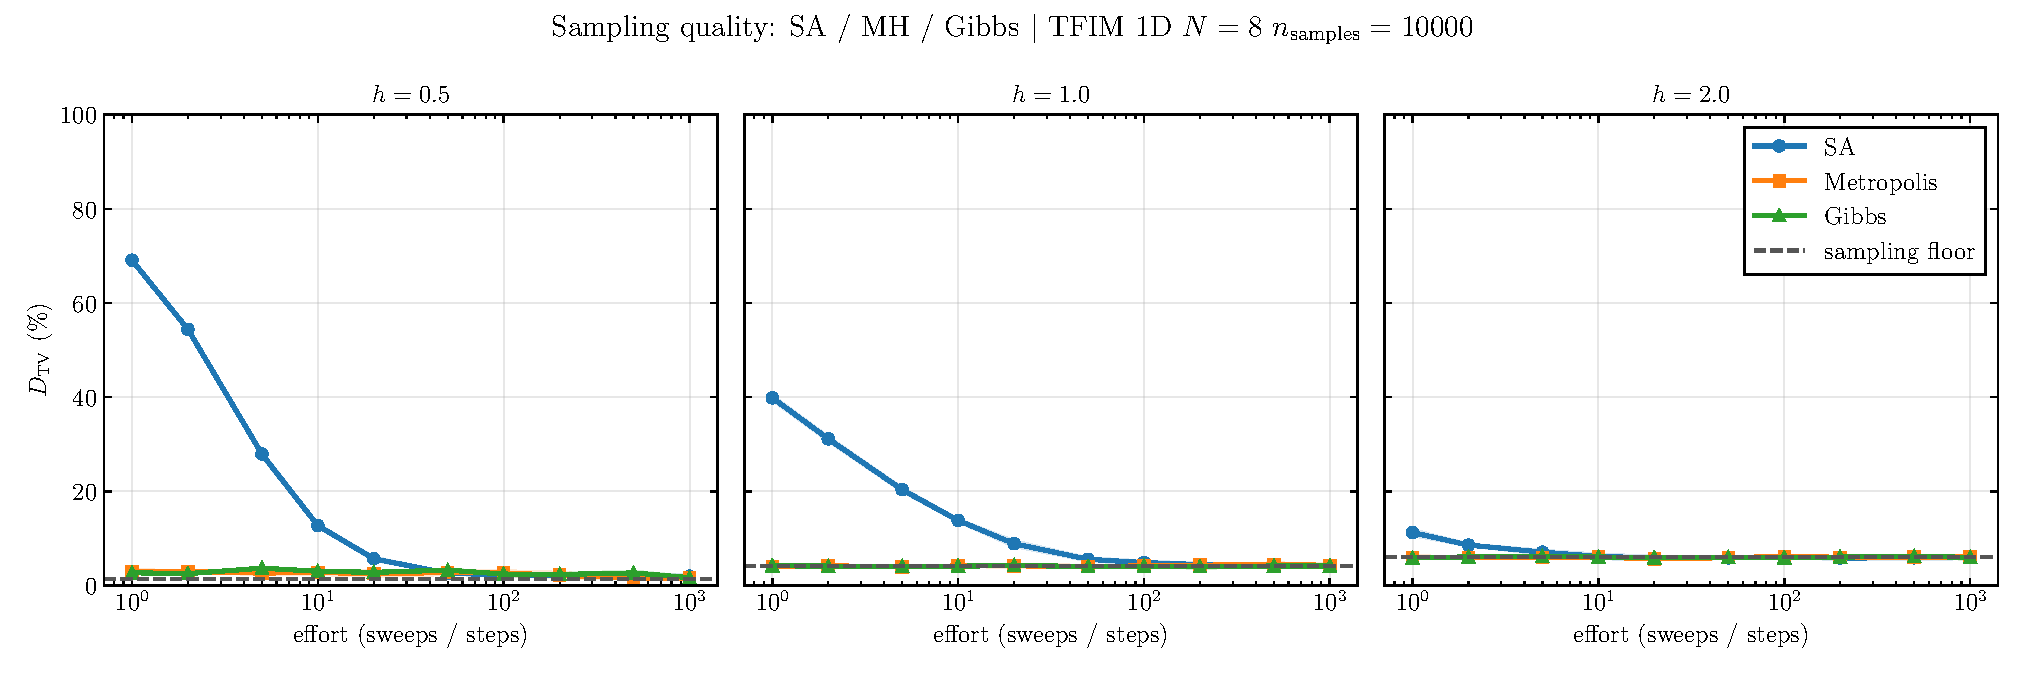
\includegraphics[width=\linewidth]{figures/dtv_classical_N8_M8.pdf}
        \caption{Total variation distance as a function of sampling effort.}
    \end{subfigure}

    \vspace{0.5em}

    \begin{subfigure}{\linewidth}
        \centering
        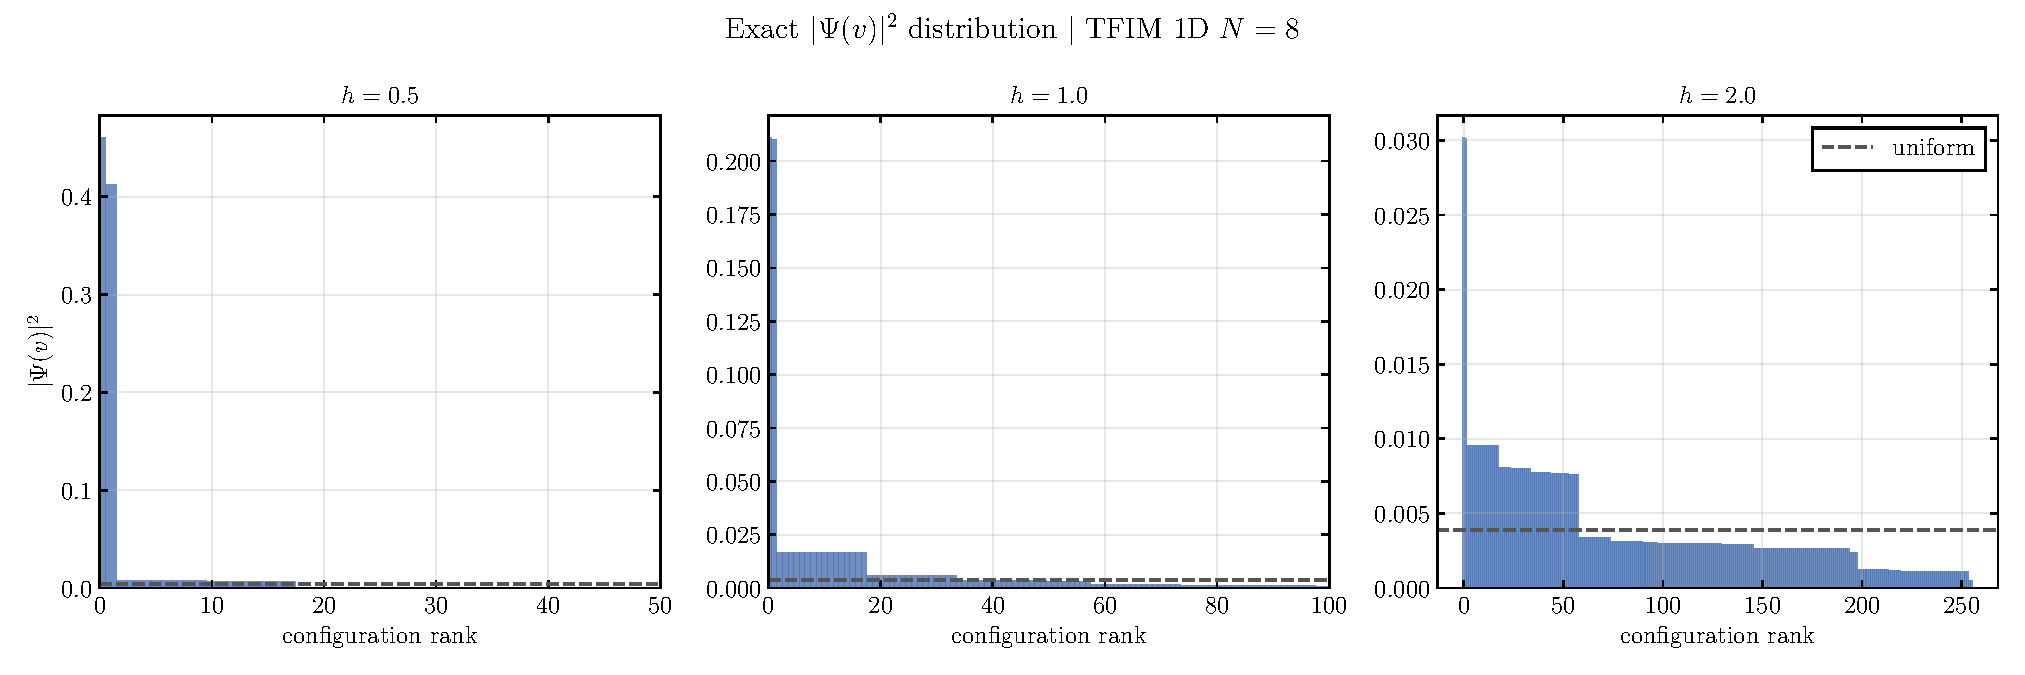
\includegraphics[width=\linewidth]{figures/dtv_classical_N8_M8_dist.pdf}
        \caption{Exact histogram of configurations.}
    \end{subfigure}

    \caption{Sampling quality for different samplers for a trained \gls{rbm} approximating the ground state of a \gls{tfim} with 8 spins, corresponding to a \gls{rbm} with 8 visible and 8 hidden units. The sampling floor is the best possible total variation distance reachable with the given number of samples. Effort is measured in sweeps.}
    \label{fig:dtv_classical_N8_M8}
\end{figure}

\begin{figure}[h]
  \centering
  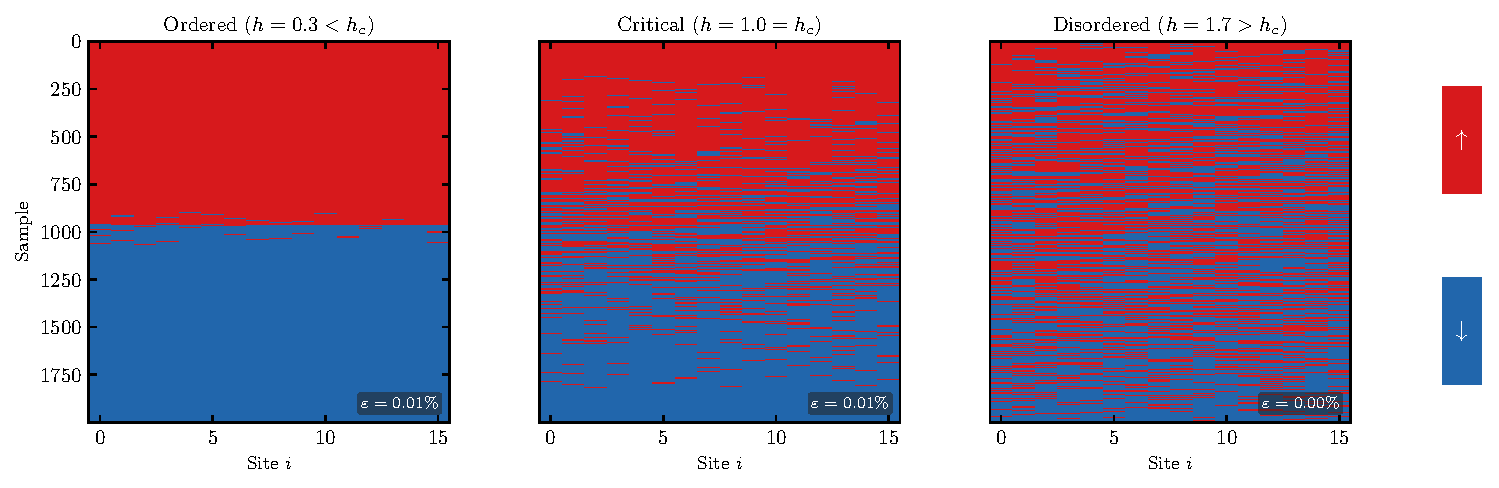
\includegraphics[width=\linewidth]{figures/spin_ordering_across_qpt}
  \caption{Spin configurations sampled from a trained RBM-VMC model for the one-dimensional Transverse-Field Ising Model (TFIM) at three values of the transverse field $h$. Each column shows 2\,000 spin configurations $\boldsymbol{\sigma} \in \{-1,+1\}^N$ sampled from the learned wave function $|\Psi_{\boldsymbol\theta}|^2$, sorted by total magnetisation. The model is a fully-connected RBM ($N = N_h = 16$) trained for 300 iterations of Stochastic Reconfiguration with 500 Metropolis-Hastings samples per step.}
  \label{fig:tfim_ordering}
\end{figure}
\subsection{Sampling temperature \& CEM}
\label{sec:exper:temp}
In this section, we evaluate the influence of temperature on different models and solvers. We focus on two quantities: the rescaling factor $\beta_x$ and the effective temperature $\beta_\text{eff}$~\cite{Benedetti_2016}. 

\subsubsection{D-Wave QPU}
The D-Wave has been found to reproduce a classical Boltzmann distribution\cite{Benedetti_2016}, parametrized by a device- and problem-dependent temperature $\beta_\text{hw}$:
\begin{equation}
p(\mathbf{v},\mathbf{h})\propto e^{-\beta_\text{hw}E_\text{in}(\mathbf{v},\mathbf{h})}
\end{equation}. Concretely, the RBM's own weights $\boldsymbol\theta=\{\mathbf{a},\mathbf{b},\mathbf{W}\}$ are divided by $\beta_x$ before being embedded on the QPU, i.e.\ $E_\text{in}=E_{\boldsymbol\theta}(\mathbf{v},\mathbf{h})/\beta_x$, so the hardware effectively samples the RBM's joint distribution at $\beta_\text{eff}=\beta_\text{hw}/\beta_x$. Therefore, all problems submitted to the QPU need to be rescaled by a factor $\beta_x$, which we estimate using \gls{cem} (described in the next section).

\label{sec:autoscale}
A common pitfall when using the D-Wave QPU is its device dependent, limited parameter range for the $h$ and $J$ values. Using the API's default settings, these parameters get automatically rescaled to fully match the allowed range. While this is not problematic for a standard minimization problem, it does impact the temperature dependent sampling process, as any temperature adjust is without effect when autoscaling is turned on.
We verify this on the \texttt{Advantage\_system6} (Pegasus) chip, using a chain-free \gls{rbm} embedded directly onto a native Pegasus biclique \autoref{fig:dtv_autoscale_N8} sweeps $\beta_x$ under both settings: with \texttt{auto\_scale=True}, the total variation distance $D_TV$ between the target and the sampled distribution stays mostly flat, as does the efficient temperature $beta_{eff}$ in \autoref{fig:dtv_autoscale_dtv_N8}. This clearly is not the case with \texttt{auto\_scale=False}, upon reaching the optimal device sampling temperature, $D_{TV}$ reduces to $\approx 30\%$. Therefore, all other D-Wave experiments in this work use \texttt{auto\_scale=False}

\begin{figure}[htbp]
    \centering
    \begin{subfigure}{0.48\linewidth}
        \centering
        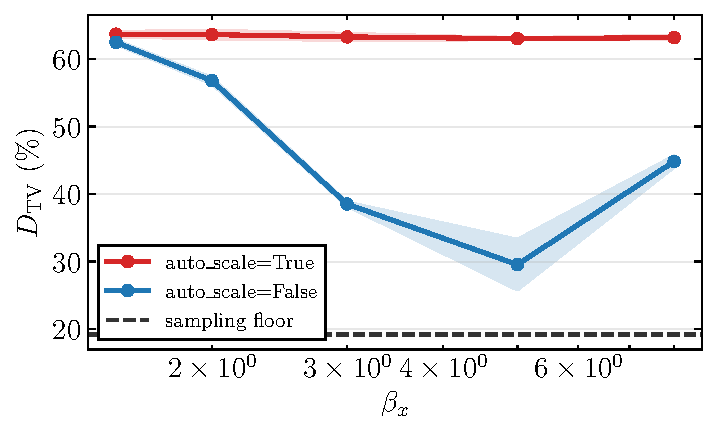
\includegraphics[width=\linewidth]{figures/dtv_autoscale_dtv_N8}
        \subcaption{Total variation distance $D_\mathrm{TV}$ between the QPU samples and $|\Psi(v)|^2$.}
        \label{fig:dtv_autoscale_dtv_N8}
    \end{subfigure}
    \hfill
    \begin{subfigure}{0.48\linewidth}
        \centering
        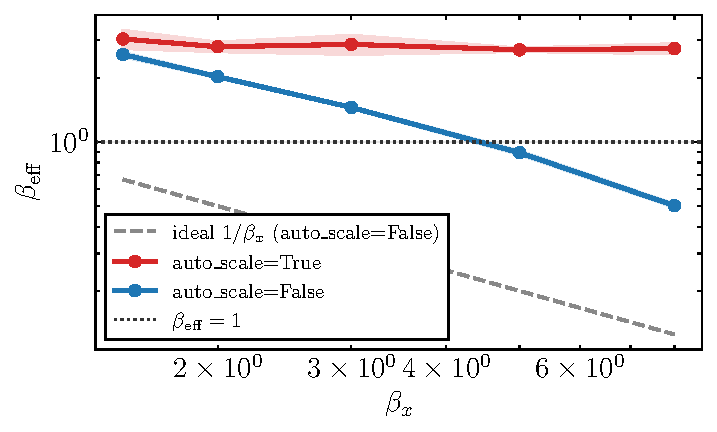
\includegraphics[width=\linewidth]{figures/dtv_autoscale_beta_N8}
        \subcaption{Effective inverse temperature $\beta_\text{eff}$, with the ideal $1/\beta_x$ line and the $\beta_\text{eff}=1$ target.}
        \label{fig:dtv_autoscale_beta_N8}
    \end{subfigure}

    \caption{%
      Impact of \texttt{auto\_scale} on $\beta_x$ for a chain-free Pegasus-embedded \gls{tfim} \gls{rbm} ($N=8$, $h=1$).}
    \label{fig:dtv_autoscale_N8}
\end{figure}
\subsubsection{CEM}
We have seen that correctly choosing the sampling temperature is crucial in obtaining meaningful distributions. \gls{cem}'s original formulation~\cite{kubo2025unlockingpowerboltzmannmachines} exploits that the hidden units of a Boltzmann machine are conditionally independent given the visible units: for a visible configuration fixed to a condition vector $\mathbf{v}=\mathbf{r}$, the conditional expectation $\langle h_j\rangle = \tanh(\beta\Theta_j)$, $\Theta_j = b_j + \sum_i r_i W_{ij}$, is known in closed form for any $\beta$. To estimate the unknown $\beta_\text{eff}$, the sampler is queried repeatedly at the fixed condition $\mathbf{r}$ to obtain an empirical conditional average $\langle h_j\rangle_{\mathbf{r},C}$, which is then matched against $\tanh(\beta\Theta_j)$ by minimizing the squared residual over $\beta$.

In this work we use a pooled variant of this matching step which reuses the joint samples $(\mathbf{v}_i,\mathbf{h}_i)_{i=1}^{N_s}$ the sampler already produces at each training iteration. We fit a single $\beta_\text{eff}$ across the whole batch,
\begin{equation}
\beta_\text{eff} = \arg\min_\beta F(\beta), \quad F(\beta) = \sum_{i=1}^{N_s}\sum_{j=1}^{N_h}\left(h_{ij}-\tanh(\beta\cdot\Theta_j(\mathbf{v}_i))\right)^2,
\end{equation}
with $i$ being the sample index. $h_{ij}$ is the observed hidden unit $j$ in sample $i$, and $\Theta_j(\mathbf{v}_i) = b_j + \sum_l v_{i,l}W_{lj}$ with $l$ the visible-unit index. This allows us to perform the CEM algorithm without additional sampling cost.

The matching step is visualized in \autoref{fig:cem_matching}, where the left subfigure shows multiple candidate functions $\tanh(\beta\Theta)$ dependent on $\beta$ that can be used to match the returned samples. The right subfigure describes the corresponding minimization, in which the squared loss function $F(\beta)$ is minimized over $\beta$ (using scipy's \texttt{minimize\_scalar} function).

For small sizes, the effective temperature $\beta_\text{eff}$ can be calculated exactly using exact enumerations. To assess the quality of the temperature estimate given by \gls{cem}, we first need to calculate the actual $\beta_\text{eff}$ numerically. This is done by first sampling from a temperature dependent sampler, follow by a minimization over $\beta$ of the KL-divergence between the sampled probability distribution and the actual, $\beta$ rescaled \gls{rbm} distribution $\nu_\beta(\mathbf v)$. This algorithm is performed over $N\in\{8,12\}$, $h\in\{0.5,1.0,1.5,2.0\}$, and $\beta_x\in\{0.5,1.0,1.5,2.0\}$ with 5 seeds and three checkpoints during training (see \autoref{fig:cem_validation}). Both subplots give the same picture: the $\beta_text{eff}$ calculated by \gls{cem} is very close to the exact solver temperature given by exact enumeration.
\begin{figure}[h]
    \centering
    \begin{subfigure}{0.48\linewidth}
        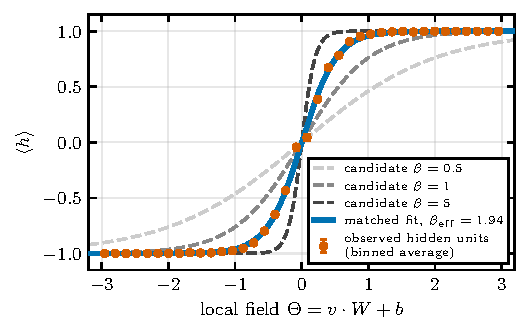
\includegraphics[width=\linewidth]{figures/cem_matching_candidates.pdf}
        \caption{Candidate fits vs.\ observed hidden units.}
        \label{fig:cem_matching_candidates}
    \end{subfigure}
    \hfill
    \begin{subfigure}{0.48\linewidth}
        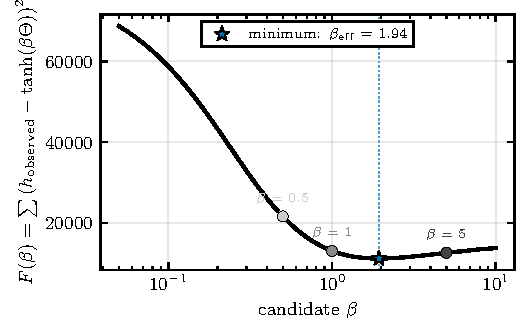
\includegraphics[width=\linewidth]{figures/cem_matching_objective.pdf}
        \caption{Matching objective $F(\beta)$.}
        \label{fig:cem_matching_objective}
    \end{subfigure}
    \caption{%
        The CEM matching step for $N=16$ spins with $h=1.0$. (a) Several candidate $\tanh(\beta\Theta)$ curves against the empirically observed hidden-unit samples. The curve at $\beta_\text{eff}=1.94$ approximates the data most closely and represents the best estimate of the sampler's temperature. (b) The squared loss function to be minimized.
    }
    \label{fig:cem_matching}
\end{figure}
\begin{figure}[h]
    \centering
    \begin{subfigure}{0.48\linewidth}
        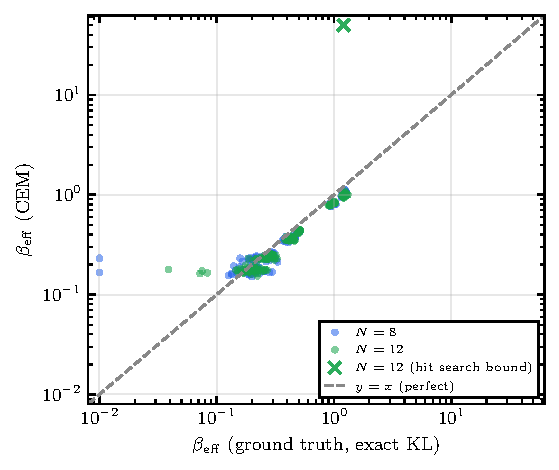
\includegraphics[width=\linewidth]{figures/cem_validation_calibration.pdf}
        \caption{CEM vs.\ exact ground truth.}
        \label{fig:cem_validation_calibration}
    \end{subfigure}
    \hfill
    \begin{subfigure}{0.48\linewidth}
        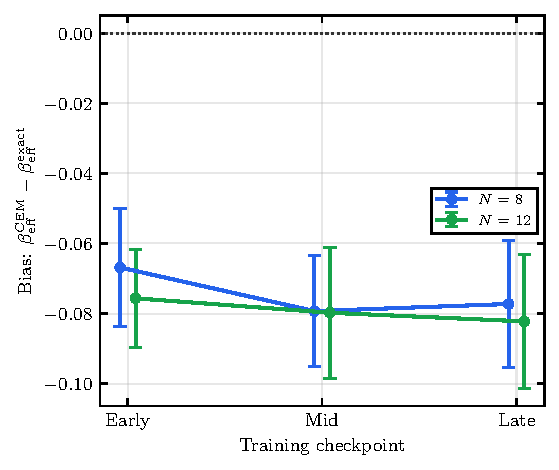
\includegraphics[width=\linewidth]{figures/cem_validation_bias.pdf}
        \caption{Bias across training.}
        \label{fig:cem_validation_bias}
    \end{subfigure}
    \caption{%
        Validation of the \gls{cem} $\beta_\text{eff}$ estimator against an exact estimate given by minimizing $D_{KL}$ against the true visible marginal of the $\beta$-rescaled joint Boltzmann distribution (a) CEM's estimate vs. the exact ground truth, the dashed lines gives the optimal values. (b) Bias of the CEM estimate relative to ground truth, averaged over $h$ and $\beta_x$, at three checkpoints during training ($10\%$/$50\%$/$100\%$ of iterations). Error bars show $95\%$ confidence intervals over seeds.
    }
    \label{fig:cem_validation}
\end{figure}


\subsubsection{Simulated Annealing}
Simulated annealing is a Metropolis-Hastings chain held at a fixed final temperature $\beta_x$; given enough sweeps it converges to the Boltzmann distribution at that temperature~\cite{Kirkpatrick_1983,Metropolis_1953}. \autoref{fig:dtv_beta_scale_N8} demonstrates this experimentally, showing $D_\mathrm{TV}$ converge toward its sampling floor as the number of cooling sweeps increases.

\begin{figure}[htbp]
    \centering
    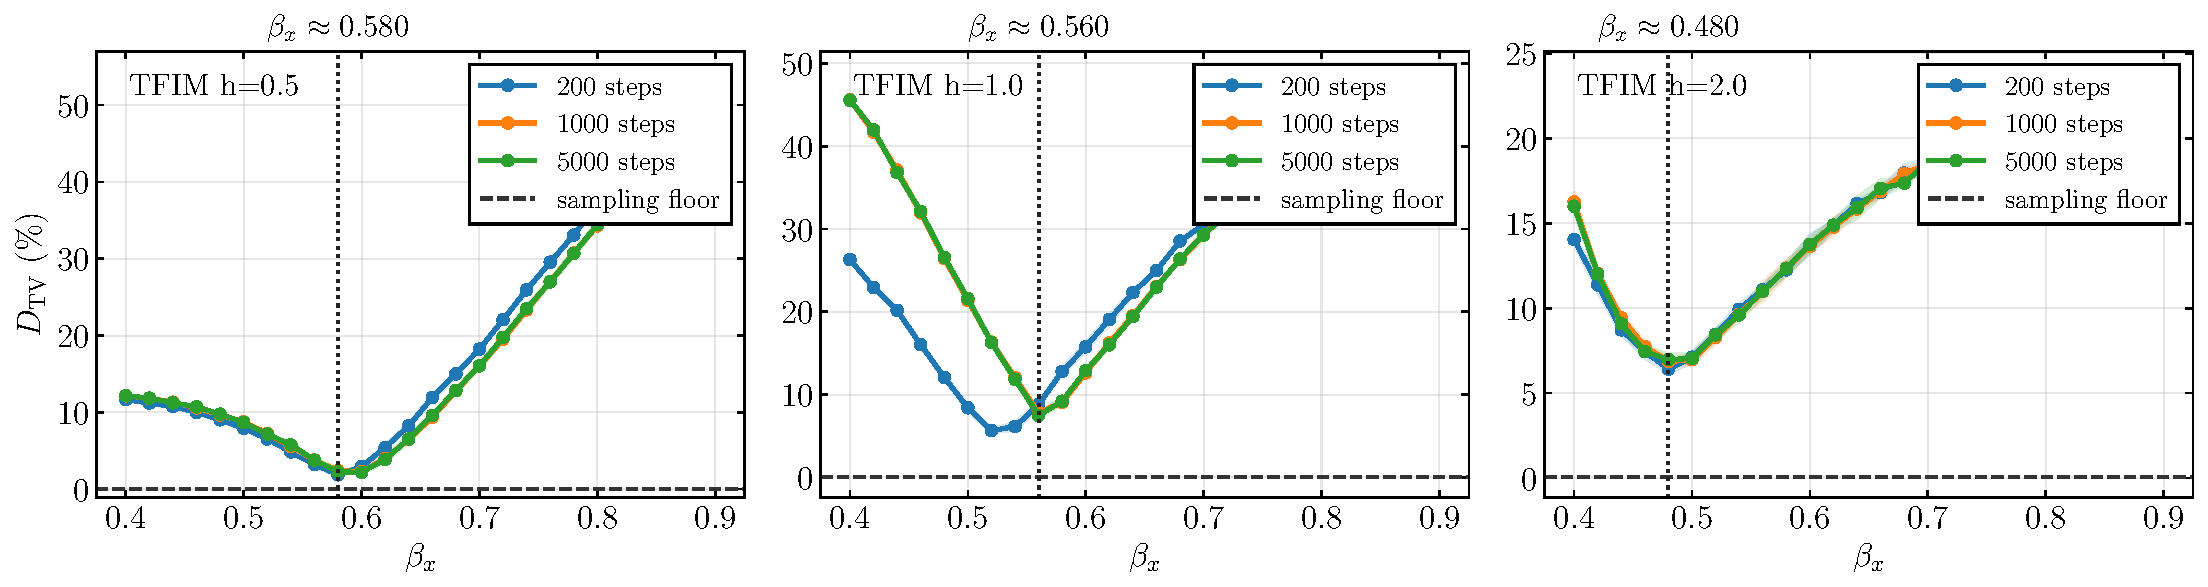
\includegraphics[width=\textwidth]{figures/dtv_beta_scale_dtv_N8}
    \caption{%
        Total variation distance $D_\mathrm{TV}$ between \gls{sa}'s empirical
        histogram and the exact distribution $|\Psi(v)|^2$, for a trained \gls{tfim} \gls{rbm} with $N=8$ visible spins, at three cooling-sweep counts.
        The horizontal dashed line marks the sampling floor; the vertical dotted line in each panel marks the $\beta_x$ that minimises $D_\mathrm{TV}$.
    }
    \label{fig:dtv_beta_scale_N8}
\end{figure}

\subsection{Improving D-Wave Topology performance}
A crucial factor in the success of an annealing process is the \textit{problem embedding} on the chip. Here, we assess two aspects related to embedding: First, introducing sparsity to fit the \gls{rbm} natively on the chip, and, second, embedding the problem multiple times to save computing time.
\subsubsection{Sparse embedding}
As described in \autoref{sec:solvers:quantum:adiab}, problems implementable on a quantum annealer often need to be fit to the QPU in an additional embedding step. We test whether a sparse, native \gls{rbm} that fits directly on the QPU performs reasonably. The sparse \gls{rbm} is created according to the following algorithm: First, construct a bipartite graph by keeping only edges that correspond to internal couplers on the D-Wave QPU. One set of the graph corresponds to visible \gls{rbm} units, the other one to hidden units. Then, greedily pick qubits for the visible units, by maximizing the overlap between neighbor sets of visible units. After all visible units are chosen, create a minimum set-cover by picking the fewest hidden qubits such that every visible qubit has at least one hidden neighbor. The remaining hidden units are filled by best connected qubits. See also \autoref{fig:sparse-embedding} for a visual overview of the algorithm.
We also look directly at the effect of sparsity on its own, keeping the number of hidden units equal to the number of visible units and only changing how many of the real couplers are removed from the connectivity mask. When removing couplers, we always remove one from the hidden unit with the highest remaining degree, so that no visible or hidden unit was ever left with zero connections. \autoref{fig:sparse-embedding} shows the resulting energy error as a function of sparsity, for three classical samplers (Metropolis-Hastings, simulated annealing, and persistent-chain Gibbs). In all three cases, error increases sharply as sparsity increases.

To establish the the best possible (theoretical) performance of a sparse \gls{rbm}, we additionally trained the same four sparsity masks ($N=16$, $h=1$, zephyr, $\alpha=1$) via exact enumeration of all $2^{16}$ visible configurations weighted by the exact $|\Psi(v)|^2$ probability, which removes all training bias from the experiment. We construct four artificial sparsity maps with the sparsity rate (the ratio of selected connection to the number of connections in a fully connected \gls{rbm}) being  $\in\{0.557, 0.682, 0.809, 0.877\}$. Making the \gls{rbm} sparser than necessary allows us to estimate the impact of a native QPU Boltzmann machine for increasing sizes of $N$, that is, the total number of spins. As can be seen in the heatmap \autoref{fig:sparsity-heatmap}, the relative error not only depends on the chosen sparsity map, but also on the $h$ value of the \gls{tfim} to be simulated. 
\begin{figure}[h]
    \centering
    \begin{subfigure}[b]{0.31\linewidth}
        \centering
        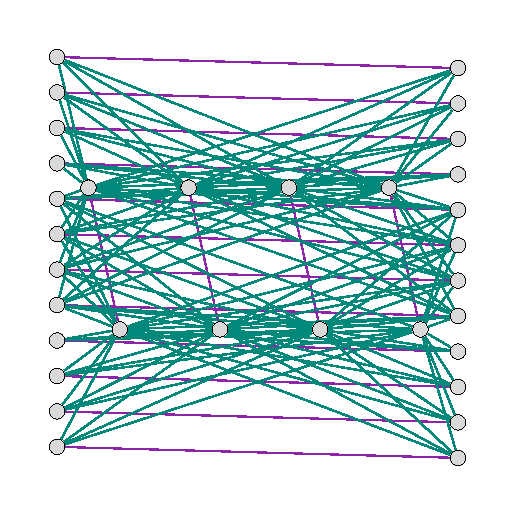
\includegraphics[width=\linewidth]{figures/sparse_graph_construction/a.pdf}
        \caption{}
        \label{fig:sparse-graph-a}
    \end{subfigure}
    \hfill
    \begin{subfigure}[b]{0.31\linewidth}
        \centering
        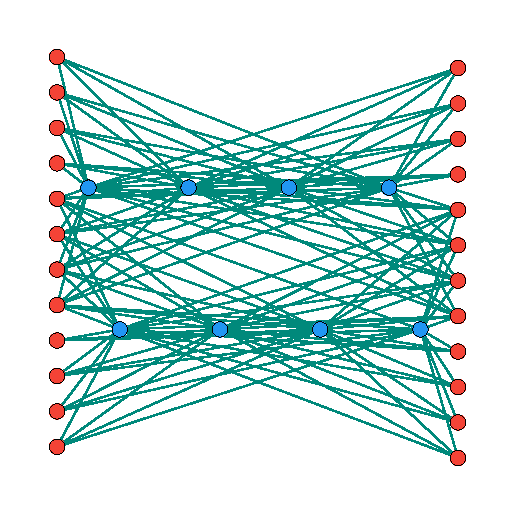
\includegraphics[width=\linewidth]{figures/sparse_graph_construction/b.pdf}
        \caption{}
        \label{fig:sparse-graph-b}
    \end{subfigure}
    \hfill
    \begin{subfigure}[b]{0.31\linewidth}
        \centering
        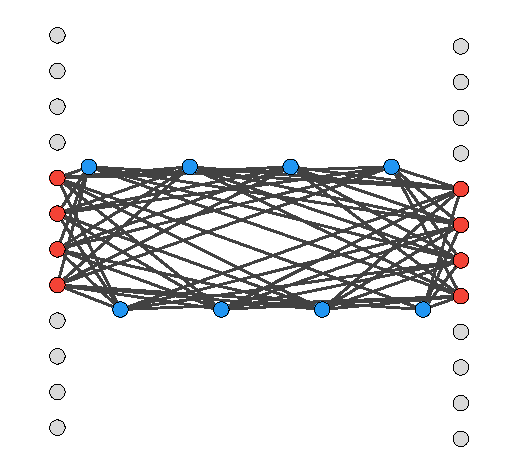
\includegraphics[width=\linewidth]{figures/sparse_graph_construction/c.pdf}
        \caption{}
        \label{fig:sparse-graph-c}
    \end{subfigure}

    \vspace{0.3em}
    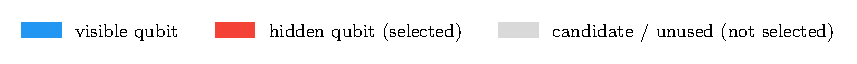
\includegraphics[width=0.6\linewidth]{figures/sparse_graph_construction/legend.pdf}

    \vspace{0.8em}
    \begin{subfigure}[b]{0.48\linewidth}
        \centering
        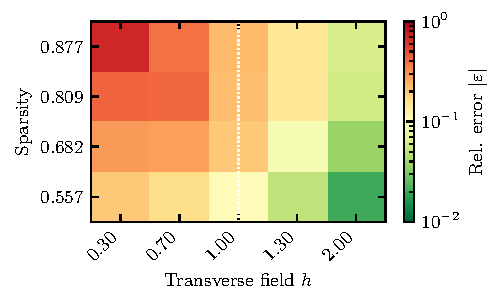
\includegraphics[width=\linewidth]{figures/sparsity/sparsity_ablation_heatmap.pdf}
        \caption{}
        \label{fig:sparsity-heatmap}
    \end{subfigure}
    \hfill
    \begin{subfigure}[b]{0.48\linewidth}
        \centering
        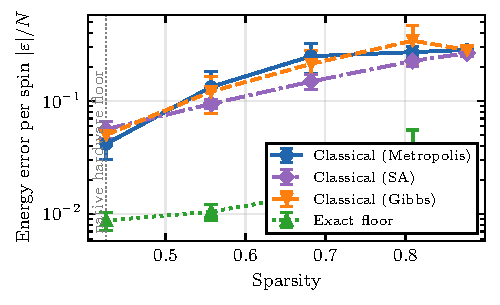
\includegraphics[width=\linewidth]{figures/sparsity/sparsity_ablation_qpu_vs_classical.pdf}
        \caption{}
        \label{fig:sparsity-line}
    \end{subfigure}

    \caption{Construction and performance of a chain-free sparse RBM from a D-Wave Zephyr hardware graph. \textbf{(a)} Identify internal couplers (green) and external/odd couplers (purple) ($N=8$ visible units shown). \textbf{(b)} Creation of bipartite graph by restricting to internal couplers, splitting into hidden unit candidates (red) and visible units (blue). \textbf{(c)} RBM's visible-hidden connectivity mask by selecting the hidden units which maximize connectivity while keeping a min-set-cover. Non-selected candidates (grey) are dropped. \textbf{(d)} Relative error $|\varepsilon|/|E_\mathrm{exact}|$ as a function of sparsity for different values of $h$, trained classically via Metropolis sampling. \textbf{(e)} Energy error per spin, $|\varepsilon|/N$, at $h=1$ across three classical samplers (Metropolis, simulated annealing, and Gibbs), against the exact-ansatz floor.}
    \label{fig:sparse-embedding}
\end{figure}
We conclude that a native Pegasus/Zephyr embedding is not suitable for efficient \gls{rbm} sampling, for the following reasons. Even in the optimal case, representability of the sparse ansatz is limited: the noise-free enumeration gives a lower bound that, in practice is hard to reach. Across three independent classical samplers (Metropolis-Hastings, simulated annealing, and persistent-chain Gibbs), trained under identical hyperparameters and iteration budgets, the per-spin error at every tested sparsity level sits $9.7$--$17.7\times$ above this floor, with no sampler avoiding the gap. Due to budget constraints, we tested the sparse models only on classical hardware.
\subsubsection{Parallel Embeddings}
To speed up calculation and save computing time, it is possible to embed multiple smaller, independent problems on the QPU~\cite{Pelofske_2022}. For example, it is possible to gather 1000 independent samples using only 250 annealing runs, by embedding the \gls{rbm} four times on the QPU. We experimentally validate this approach with 3 seeds per $n_\mathrm{parallel} \in \{1,3,5\}$, as \autoref{fig:parallel-embedding} makes visible that training at this iteration budget is not reliable: 4 of the 9 runs diverge (crossed-off markers), including 2 of 3 seeds at $n_\mathrm{parallel}=5$. For the runs that do converge, \autoref{fig:parallel-embedding-qpu-time} indicates that parallel embedding can indeed be used to save QPU time. To find a parallel embedding, we use D-Wave's \texttt{dwave.system.ParallelEmbeddingComposite}.
\begin{figure}[h]
    \centering
    \begin{subfigure}[b]{0.48\textwidth}
        \centering
        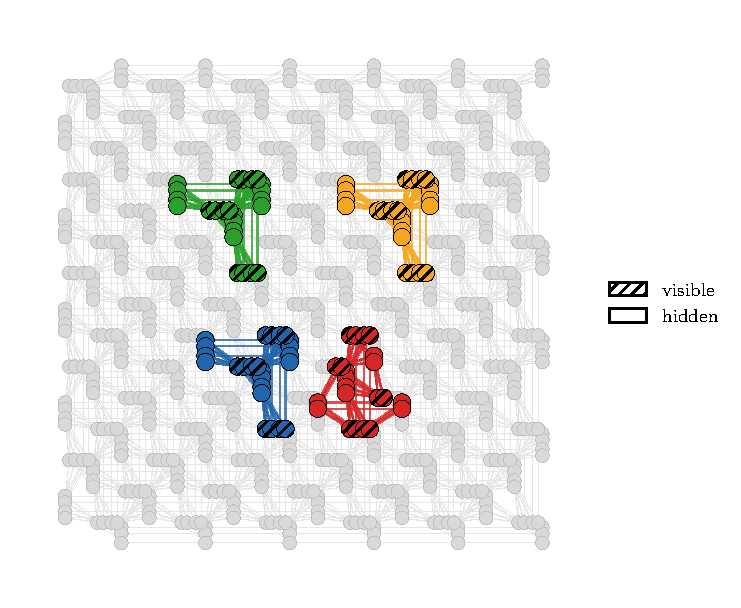
\includegraphics[width=\textwidth]{figures/parallel_embedding/parallel_embedding_np4_pegasus.pdf}
        \caption{Four independent $K_{8,8}$ RBM embeddings ($n_\mathrm{parallel}=4$) placed simultaneously on the Pegasus chip. Colors distinguish copy 1-4; hatched markers denote visible units, solid markers denote hidden units.}
        \label{fig:parallel-embedding-chip}
    \end{subfigure}
    \hfill
    \begin{subfigure}[b]{0.48\textwidth}
        \centering
        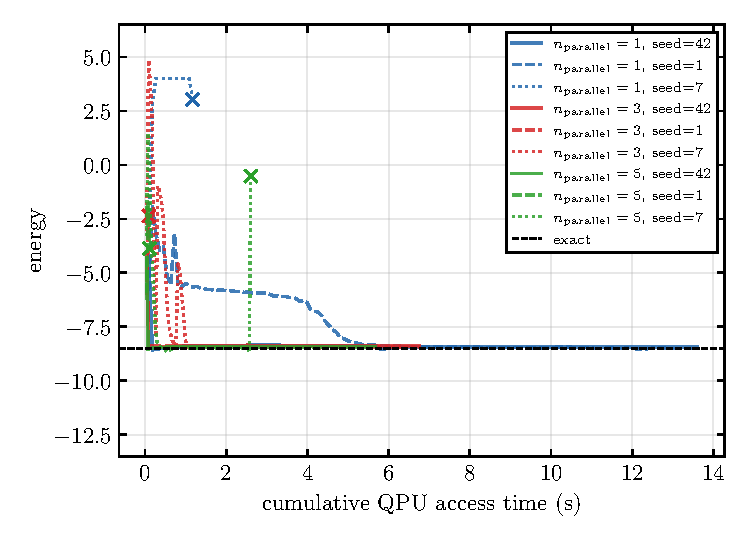
\includegraphics[width=\textwidth]{figures/parallel_embedding/parallel_embedding_np_seeds_qpu_time.pdf}
        \caption{Energy vs.\ cumulative QPU access time for $n_\mathrm{parallel} \in \{1,3,5\}$, all 3 seeds shown individually. $\times$ markers indicate a run diverged before reaching the plateau.}
        \label{fig:parallel-embedding-qpu-time}
    \end{subfigure}
    \caption{Parallel embedding on a D-Wave QPU: (a) physical embedding layout, (b) resulting training speedup.}
    \label{fig:parallel-embedding}
\end{figure}
\subsection{Sign Problem in Quantum Monte Carlo}
It is well known that capturing some quantum dynamics with non-trivial sign structure using a real-valued variational ansatz is not possible (\textit{sign problem}). This does not pose a problem for the \gls{tfim} models, as it is a \textit{stoquastic} model\cite{2011772.2011773}. A stoquastic matrix is defined to have only real and non-positive off-diagonal elements. It can easily be seen that the \gls{tfim} is stoquastic from its definition in  \autoref{eq:tfim}: the $\sigma^z_i\sigma^z_j$ terms only contribute diagonal elements, and the off-diagonal elements from the tranverse field $\sigma^x_i\sigma^x_j$ all contribute the same factor $-h$. Some Heisenberg $J1-J2$ models do not have this property and the corresponding \gls{rbm} training converges far from the ground state (see \autoref{fig:convergence_median}). 

The reason for this is that the factors  $e^{-\mathbf{a}\cdot\mathbf{v}/2}$ and $\cosh(\cdot)$ of the \gls{rbm} ansatz defined in \autoref{eq:ansatz} are strictly positive for real parameters and therefore the ansatz does not allow for the representation of negative amplitudes. 
\subsubsection{Marshall sign rule}
\label{sec:marshall}
\paragraph{Non-stoquasticity of the Heisenberg model} To understand why the sign problem appears in the Heisenberg model and not in the \gls{tfim}, we need to assess the off-diagonal values of the system Hamiltonian. Writing a bond between sites $i$ and $j$ as $H_{ij}=J[\sigma^x_i\sigma^x_j+\sigma^y_i\sigma^y_j+\sigma^z_i\sigma^z_j]$, only the $\sigma^x_i\sigma^x_j+\sigma^y_i\sigma^y_j$ part is off-diagonal (it flips both spins of an antiparallel pair, e.g.\ $\ket{\uparrow\downarrow}\to\ket{\downarrow\uparrow}$), while $\sigma^z_i\sigma^z_j$ leaves the configuration unchanged. Using $\sigma^x\ket{\uparrow}=\ket{\downarrow}$, $\sigma^y\ket{\uparrow}=i\ket{\downarrow}$, and $\sigma^y\ket{\downarrow}=-i\ket{\uparrow}$, the two terms act on the antiparallel pair as
\begin{equation}
\left(\sigma^x_i\sigma^x_j+\sigma^y_i\sigma^y_j\right)\ket{\uparrow\downarrow} = \ket{\downarrow\uparrow} + (i)(-i)\ket{\downarrow\uparrow} = 2\ket{\downarrow\uparrow},
\end{equation}
Consequently, every antiparallel bond contributes
\begin{equation}
\bra{\downarrow\uparrow}H_{ij}\ket{\uparrow\downarrow}=2J.
\end{equation}
To restore stoquasticity, it is enough to simply multiply the off-diagonal elements $E_\text{loc}$ contribution by $-1$. This can be motivate by the Marshall sign rule~\cite{Marshall_1955}, which can be used to remove the non-trivial sign structure of the ground state wavefunction by basis transformation. Considering the following unitary transformation on bipartite lattices $A \cup B$ (two sublattices such that every nearest-neighbour bond connects a site in $A$ to one in $B$, as on an alternating chain), written in the Pauli convention:
\[
U = \prod_{i \in A} \sigma_i^z,
\]
the ground state wavefunction can be written as
\[
U |\psi_0\rangle = \sum_{\sigma} |c_\sigma| \, |\sigma\rangle,
\]
with only positive amplitudes. This flip is exact for every $J_1$ bond, since bipartiteness guarantees each one connects $A$ to $B$. A $J_2$ bond, however, connects two sites of the \emph{same} sublattice so $U$ leaves its sign unchanged. The correction is therefore exact only for $J_2=0$. It has however been shown that the Marshall correction can survive a certain degree of frustration (i.e.\ for $J_2/J_1$ up to a certain threshold)\cite{Richter_1994,Voigt_2000}, which we validate experimentally.

\begin{figure}[htbp]
    \centering
    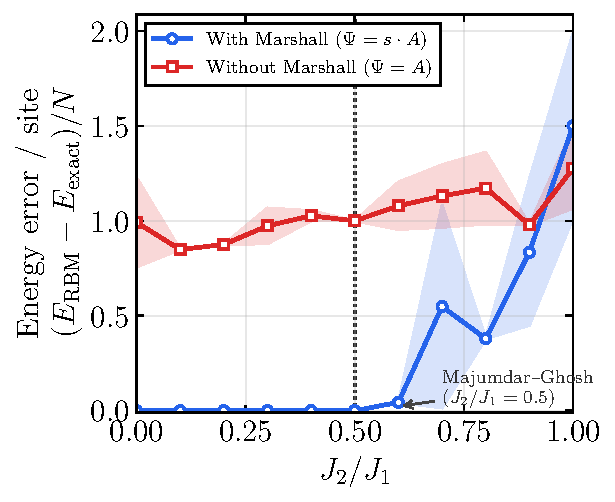
\includegraphics[width=0.75\linewidth]{figures/marshall_comparison/marshall_comparison_energy.pdf}
    \caption{Energy error per site, $|E_\text{RBM}-E_\text{exact}|/N$, with and without the Marshall sign correction, against $J_2/J_1$ (mean $\pm$ std over seeds). Model trained using Metropolis-Hastings sampling, $N=8$, 200SR iterations and averaged over 3 seeds, swept over 11 points from $0$ to $1$.}
    \label{fig:marshall-comparison}
\end{figure}

We validate this experimentally in \autoref{fig:marshall-comparison}: applying the Marshall sign correction reduces the ground-state energy error by several orders of magnitude compared to the uncorrected ansatz, confirming that the correction works in practice. Consistent with \cite{Richter_1994}'s square-lattice result and \cite{Voigt_2000}'s direct calculation for the 1D chain, this improvement persists over a range of frustration $J_2/J_1$ before degrading, verifying that the sign rule can empirically survive frustration beyond its proven regime of $J_2=0$. We did not test a phase-capable ansatz (e.g.\ a complex-valued \gls{rbm}) and leave it to future work.
\begin{figure}[htbp]
    \centering
    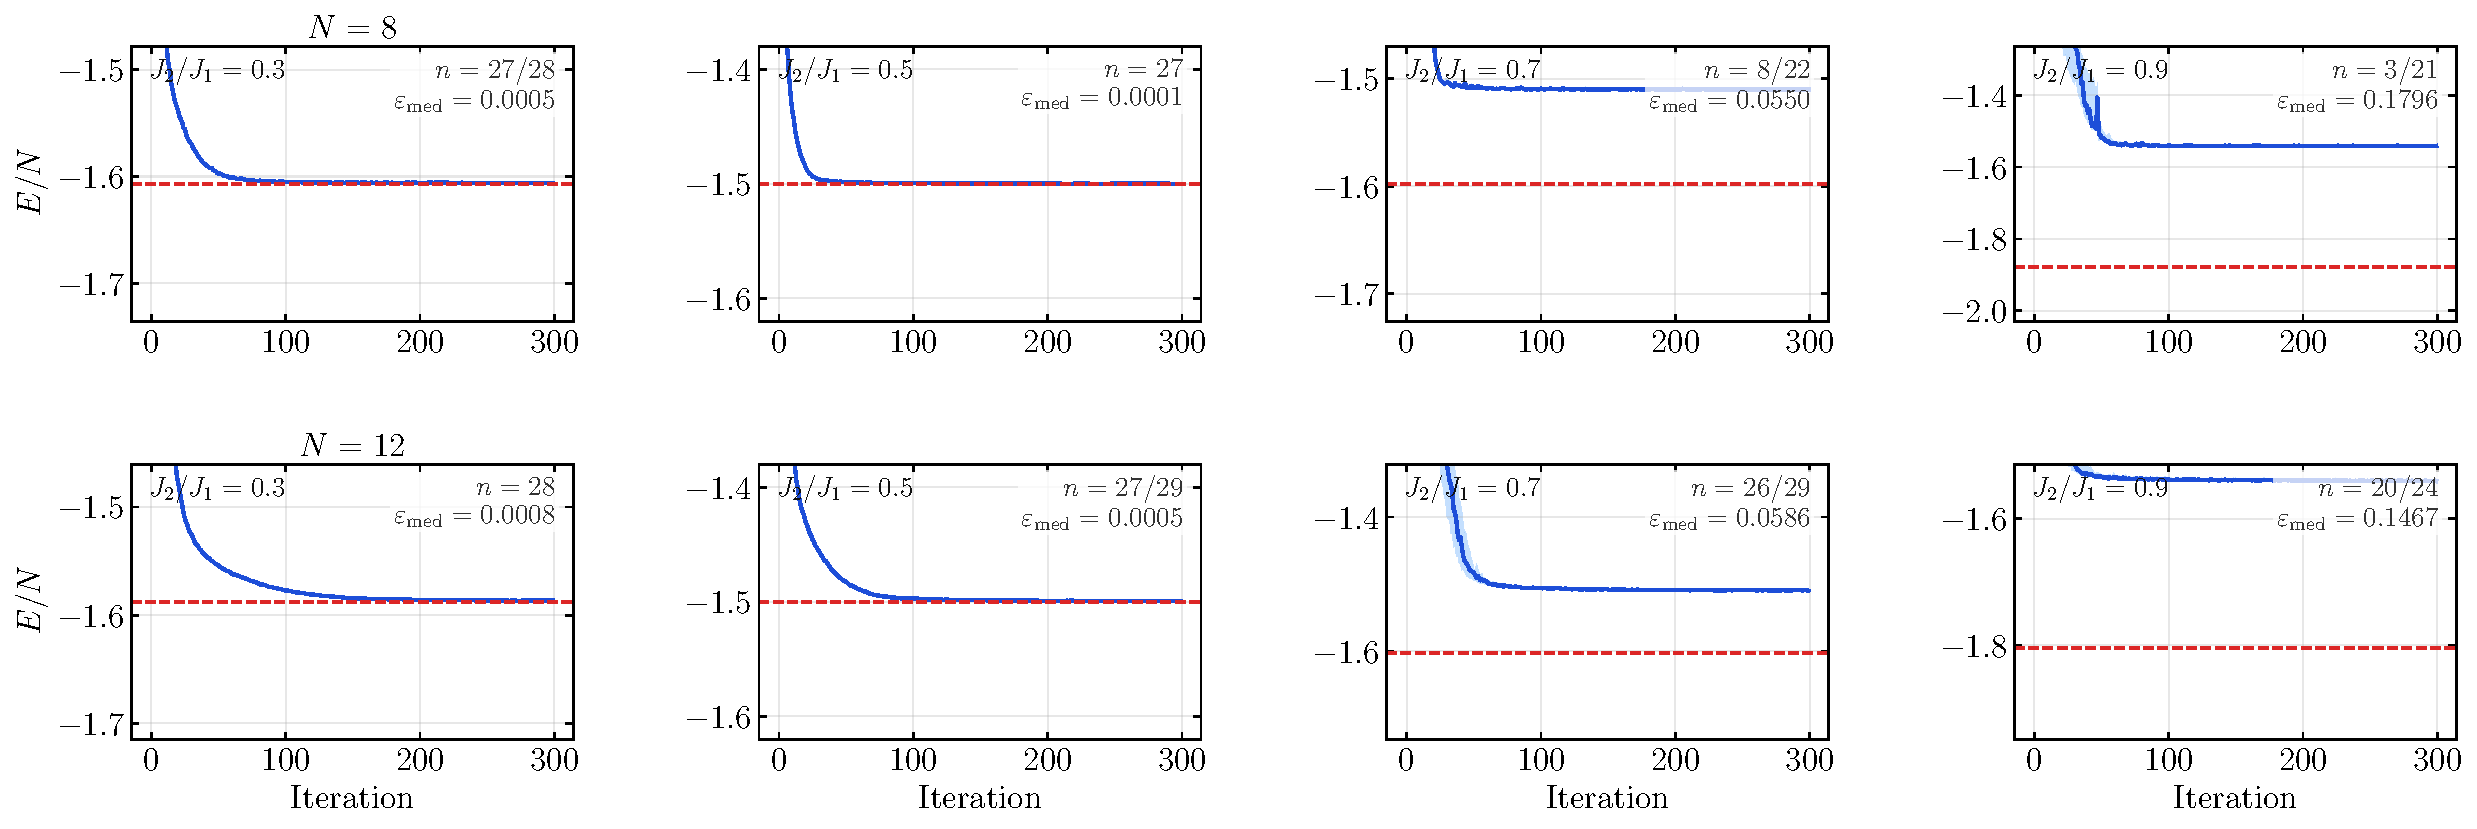
\includegraphics[width=\linewidth]{figures/fig_convergence_median.pdf}
    \caption{RBM convergence curves ($E/N$ vs.\ SR iteration) for
    $N \in \{8,12\}$ and $J_2/J_1 \in \{0.3,0.5,0.7,0.9\}$ on the frustrated $J_1$--$J_2$ Heisenberg chain, using Gibbs sampling. The solid line is the median over $n$ independent evaluation seeds, the shaded band is the interquartile range. Where $n$ is reported as $a/b$, $b$ seeds were attempted and $b-a$ runs diverged under the selected configuration divergence is frequent in the strongly frustrated regime ($N=8$, $J_2/J_1 \geq 0.7$). The red dashed line marks the exact ground-state energy $E_\mathrm{exact}/N$.}
    \label{fig:convergence_median}
\end{figure}

\subsection{Time-to-$\epsilon$ across solvers}
\label{sec:exper:tte}
\subsubsection{Methodology}
We present a hyperparameter matched solver comparison for the one-dimensional \gls{tfim} with $h=0.5$ for $N$ up to 64. Solvers are compared by pure sampling time only, that is without taking into account the classical training iteration overhead (i.e. \gls{sr} calculation, which is identical across solvers). All runs are performed using the same hyperparameters ($N$ hidden units (matching the visible count), learning rate $0.08$, regularization $0.05$, $200$ samples per iteration, a $100$-iteration budget, and $20$ seeds per cell) and solver dependent internal parameters, which can be found in \autoref{tab:classical_sampler_params}. For the D-Wave in particular, only the QPU's own \texttt{qpu\_access\_time} (on-chip programming, anneal, and readout) is taken into account as returned by D-Wave's SAPI, one-time embedding and per-sampler network latency are excluded. For the classical solvers a separate one-time call is executed before training starts to trigger JAX's \gls{jit} compilation, so that cost is excluded from every reported iteration. 

We report on \gls{tte}$_{99}$: following the same $99\%$-confidence convention already used for \gls{tts} in \autoref{eq:tts}, the expected time for a run to reach the solution to within a given energy tolerance $\epsilon$ with $99\%$ confidence, computed from the validated (successful) fraction of seeds and their convergence time. The precise definition is given below.

A run is considered to converge when the rolling-window mean energy error per spin, $|\overline{E}-E_\mathrm{exact}|/N$ averaged over the trailing $10$ iterations, first drops below $\epsilon=0.1$ and stays below it for $10$ consecutive iterations. A run that does not satisfy this criterion within the $100$-iteration budget is censored, i.e.\ does not validate. Pegasus and Zephyr are reported here with \gls{cem} correction only; for these series, the reported time also includes \gls{cem}'s $\beta_\text{eff}$ estimation step which is added on top of the QPU's own device-reported \texttt{qpu\_access\_time}.

Formally, with $E_\tau$ the training energy logged at \gls{sr} iteration $\tau$, window size $w=10$, and iteration budget $T=100$, the rolling-window mean and its error are
\begin{equation}
\label{eq:tte-window}
\overline{E}_t = \frac{1}{t - t_0 + 1}\sum_{\tau=t_0}^{t} E_\tau, \qquad t_0 = \max(1,\, t-w+1), \qquad
\delta_t = \frac{\big|\overline{E}_t - E_\mathrm{exact}\big|}{N}.
\end{equation}
The convergence iteration is the first sustained crossing for $w$ iterations,
\begin{equation}
\label{eq:tte-conv}
t^\star = \min\Big\{\, t \le T-w+1 \;:\; \delta_s < \epsilon \ \ \forall\, s \in \{t,\dots,t+w-1\} \,\Big\},
\end{equation}
undefined (censored) if no such $t^\star$ exists within budget. For a given solver and $N$, let $p$ be the fraction of the $20$ seeds for which $t^\star$ exists (validate), and let
\begin{equation}
\label{eq:tte-Tr}
T_r = \operatorname{median}_{\text{validated seeds}} \ \sum_{\tau=1}^{t^\star} s_\tau
\end{equation}
be the median wall-clock convergence time of those validated seeds ($s_\tau$ the time for one sampler call, so the sum is the cumulative sampling time up to and including iteration $t^\star$). Analogously to \gls{tts} (\autoref{eq:tts}), a run that fails to validate is treated as a failure to be retried from scratch with a new seed, giving the $99\%$-confidence
\begin{equation}
\label{eq:tte99}
\mathrm{TTE}_{99} =
\begin{cases}
T_r, & p = 1, \\[2pt]
T_r \dfrac{\ln(1-0.99)}{\ln(1-p)}, & 0 < p < 1, \\[4pt]
\text{undefined (censored)}, & p = 0.
\end{cases}
\end{equation}
The same conversion, applied to the IQR bounds of the validated seeds' convergence times instead of their median, gives the reported \gls{tte}$_{99}$ error bars.


\subsubsection{Results analysis}
\autoref{fig:tte_self_convergence} (top) plots the median \gls{tte}$_{99}$ (with interquartile range) against system size $N\in\{8,12,16,24,32,64\}$ on three panels: \textbf{(a)} classical MCMC samplers (Metropolis, Gibbs); \textbf{(b)} classical, physics-inspired heuristics (\gls{sa} run locally on the GPU described in \autoref{sec:hw_config}, and FPGA); and \textbf{(c)} the Pegasus and Zephyr QPUs with \gls{cem} correction. For budget reasons, we report QPU results at four sizes only: $N\in\{8,16,32,64\}$. 

FPGA is fastest through $N=32$, where every series still validates $20/20$ seeds and \gls{tte}$_{99}$ therefore equals $T_r$ (no retries needed, $p=1$). By $N=64$, however, a handful of seeds no longer validate within budget for several series (FPGA $19/20$, Zephyr(+CEM) $19/20$, Metropolis $17/20$, Gibbs $16/20$, \gls{sa} $18/20$): FPGA's \gls{tte}$_{99}$ ($0.87\,\mathrm{s}$) is now clearly higher than Pegasus(+CEM)'s ($0.47\,\mathrm{s}$, still $20/20$ validated at every size). Gibbs stays essentially flat across $N$ (its lowest fitted exponent, $\propto N^{+0.65}$) since its dominant cost is a fixed one-time $200$-sweep persistent-chain initialization (\autoref{tab:classical_sampler_params}), which does not grow with $N$ in this range; Metropolis and \gls{sa} have no such fixed cost and grow steeply instead. 

\autoref{fig:tte_self_convergence} (bottom) reports the same validated-convergence cells in terms of GPU energy consumed instead, restricted to classical solvers. The D-Wave QPUs are omitted because no reliable energy consumption value could be established. FPGA energy is an assumed-constant-power estimate ($45\,\mathrm{W}$).

\begin{figure}[h]
    \centering
    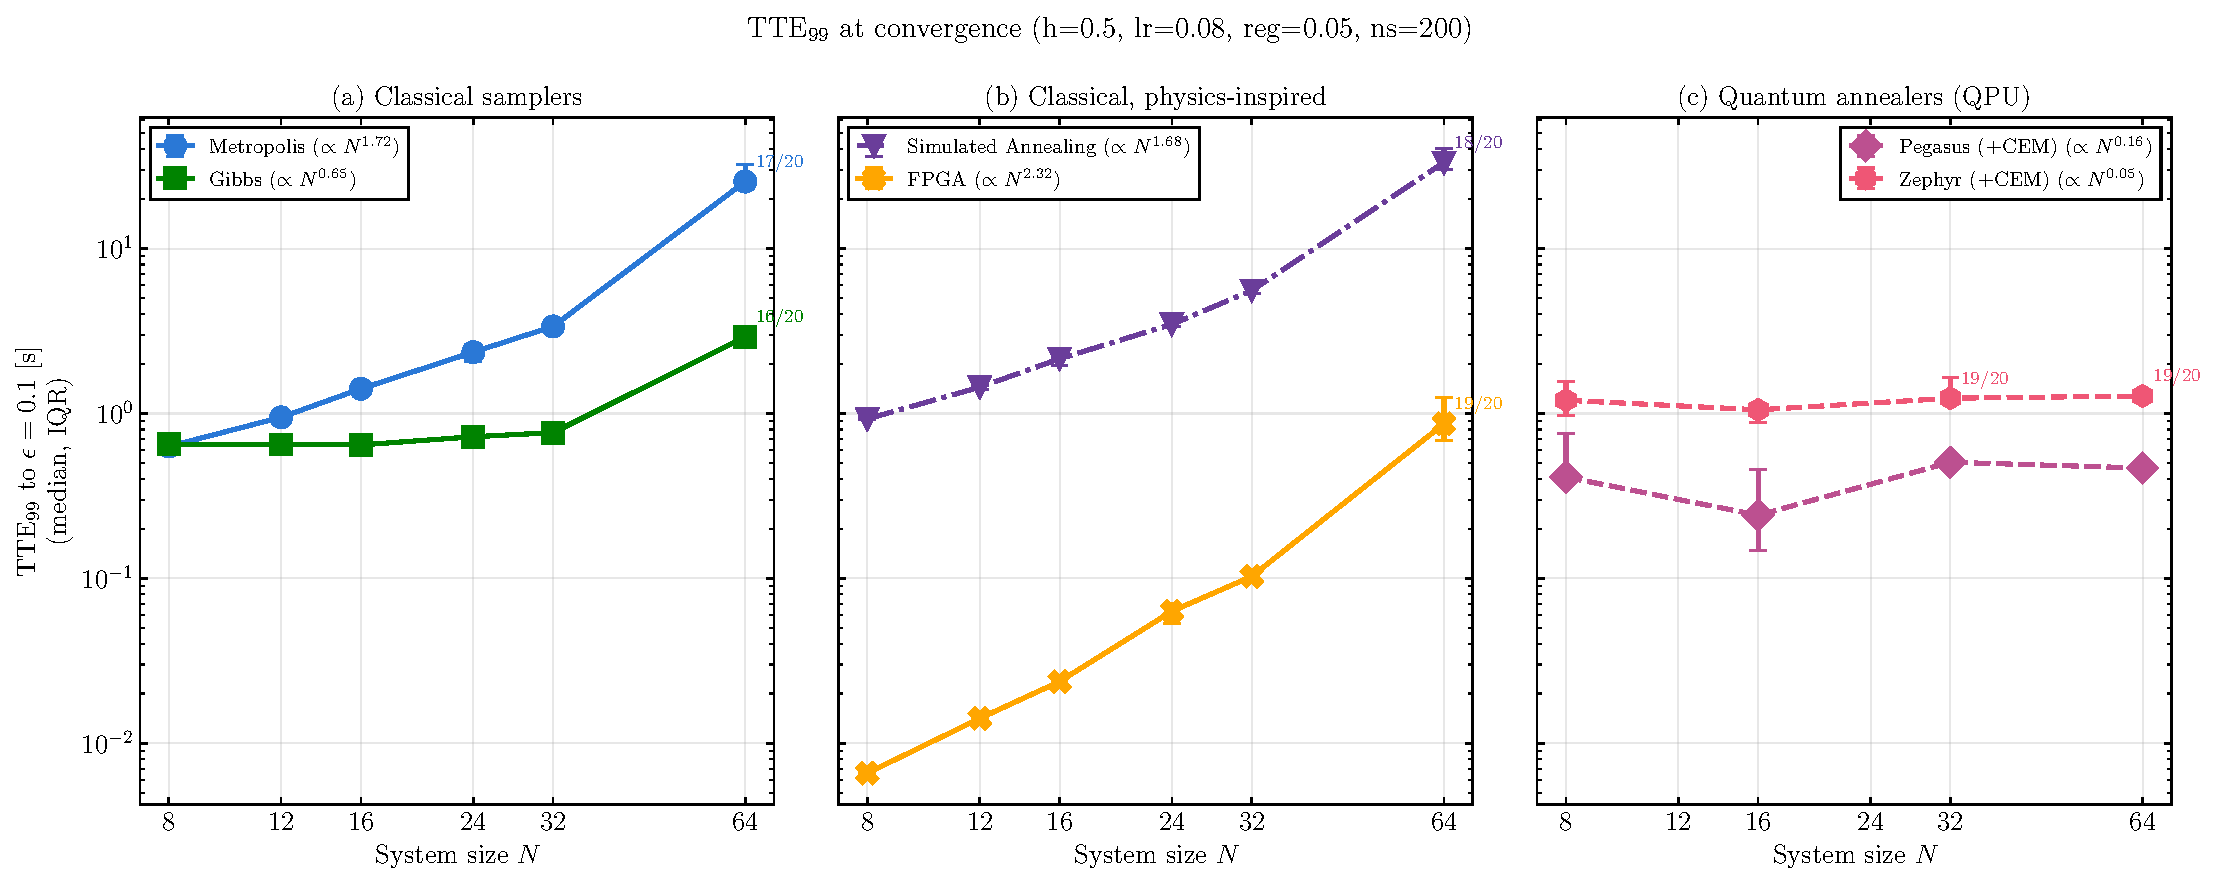
\includegraphics[width=\linewidth]{figures/fig10c_tte99_vs_n_eps0.1.pdf}
    \par\vspace{1.2em}
    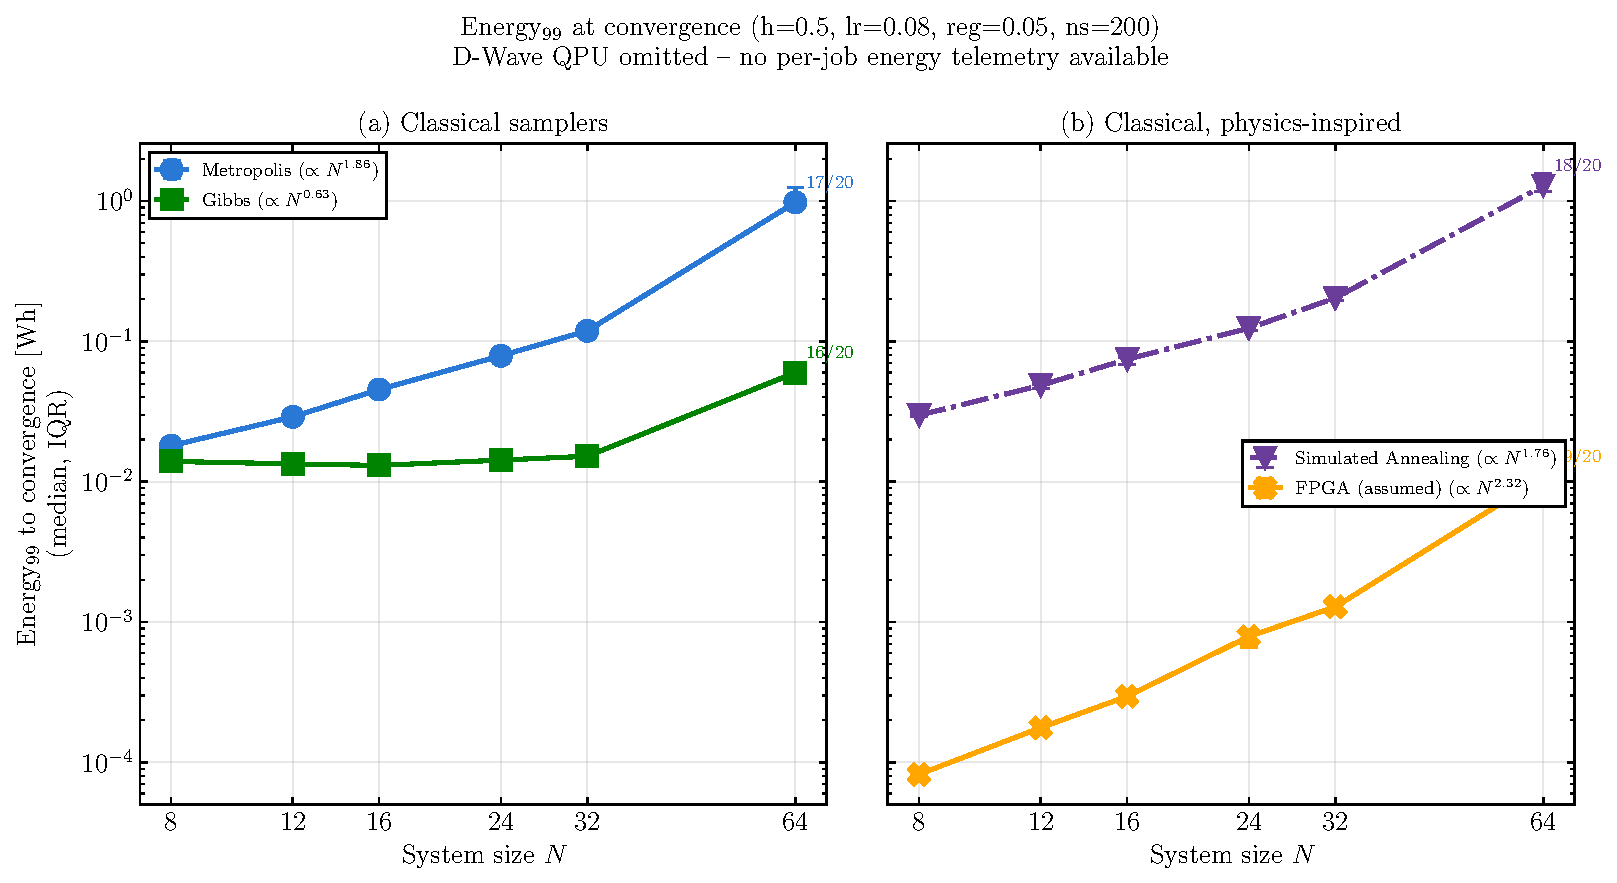
\includegraphics[width=0.75\linewidth]{figures/fig10d_energy99_vs_n_eps0.1.pdf}
    \caption{\textbf{(top)} Median \gls{tte}$_{99}$ (interquartile range) against system size $N$, under the protocol given in the text. Panels: \textbf{(a)} classical samplers, \textbf{(b)} classical physics-inspired heuristics, \textbf{(c)} quantum annealers (QPU, with \gls{cem} correction; raw QPU access time omitted, see text). Markers are annotated with the validated-over-total seed count whenever that fraction is below $20/20$. Dotted lines show each series' fitted power law $\propto N^p$, with $p$ given in the legend. \textbf{(bottom)} Median GPU energy$_{99}$ to the same validated-convergence cells, panels (a)--(b) only}
    \label{fig:tte_self_convergence}
\end{figure}

\section{Conclusion}
We assessed classical, quantum-annealing, and physics-inspired samplers within one framework, across the transverse-field Ising and Heisenberg models, using both time-to-solution and energy consumption. FPGA is the fastest and most energy-efficient of the metered classical solvers; QPU energy was not measured, so no classical-versus-quantum energy comparison is claimed. On time-to-solution, Pegasus(+\gls{cem}) becomes statistically indistinguishable from FPGA by $N=64$; only Zephyr(+\gls{cem}) shows a weak favorable trend, not robust enough across the criterion's parameters to claim general quantum competitiveness. Native sparse embedding onto the annealer's hardware graph costs more accuracy than it saves in overhead; parallel embedding of multiple problem copies is a promising direction, but the seed count collected here is too small to support a quantitative speedup claim. The variational ansatz cannot represent ground states with sign structure; the Marshall sign rule restores good accuracy for weakly frustrated Heisenberg chains, but accuracy degrades beyond moderate frustration. Overall, physics-inspired classical hardware remains the strongest sampler at current scale; the QPU's scaling behavior is mixed across encodings and not strong enough, on its own, to support a general claim of future competitiveness.

% -------------------- Appendix -------------------- *
\clearpage
\section{Appendix}
\subsection{JAX}
\label{sec:jax}
(Quantum) variational algorithms do not only strain \textit{quantum} resources, but also push \textit{classical} computers to their limits. Notably, at each iteration, the stochastic reconfiguration process described in \autoref{sec:stochsticreconfig} adapts all parameters of the weights and biases. We use several techniques in this project to speed up this process. JAX, implementing the \textit{functional programming} paradigm, allows for the speed up of function calls and linear algebra calculation by offering features such as \gls{jit} compilation and XLA (accelerated linear algebra). We will describe the features of JAX in detail and give examples from our codebase.
\subsubsection{Just-in-time compilation}
JAX transformations require functions to be \textit{functionally pure}. To summarize, a function is considered functionally pure, if its output depends only on the function's input parameters, and all output is passed through the return variable. As an example, a function that involves \texttt{print()} statements or writes to global variables is not considered to be functionally pure, as its output does not exclusively pass through the \texttt{return} statement. JAX does not guarantee the proper behavior of impure functions. During \gls{jit} compilation, the function is transformed to primitives, which in JAX are defined to be "fundamental units of computation"\cite{jaxGlossaryTerms}. As an example, the following function header is used to calculate the local energy (\autoref{eq:localenergy}):

\begin{lstlisting}[language=Python]
  @functools.partial(jax.jit, static_argnums=(4, 5))
  def _local_energy_1d_jit(
      V: jax.Array,  # (ns, N) -- spin configs
      W: jax.Array,  # (N, M)  -- RBM weights
      a: jax.Array,  # (N,)    -- visible biases
      b: jax.Array,  # (M,)    -- hidden biases
      h: float,      # static
      N: int,        # static
  ) -> jax.Array:    # (ns,)   local energies
      ...
  \end{lstlisting}
$h$ and $N$ are passed as static parameters, meaning that they will be hard-coded in the compiled function after \gls{jit}. JAX compiles a kernel for each combination of static variables; as $h$ and $N$ never change during a training run, this means that the function is only compiled once.

\subsubsection{Vectorized Map}

\texttt{jax.vmap} takes a function written for a single input and returns a new function that maps it over a leading batch axis as a single vectorised kernel.

As a concrete example, consider \texttt{log\_psi\_fn} defined for a single spin configuration $\mathbf{v} \in \{-1,+1\}^N$. Evaluating it over all $n_s$ sampled configurations reduces to:

\begin{lstlisting}[language=Python]
log_p_V = jax.vmap(log_psi_fn)(V)   # V: (ns, N) -> log_p_V: (ns,)
\end{lstlisting}

XLA compiles this as a single operation over the batch dimension rather than $n_s$ independent kernel launches. The resulting operation can be compiled using \gls{jit} for faster execution:

\begin{lstlisting}[language=Python]
batched_f = jax.jit(jax.vmap(log_psi_fn))
\end{lstlisting}

JAX also offers automatic differentiation, but we do not use it, since gradients are calculated analytically (see \cite{Gardas_2018}).

\subsection{Hardware and Software Configuration}
\label{sec:hw_config}
All classical computation (classical and training loop) run locally via JAX on a single NVIDIA TITAN RTX GPU (24\,GB, driver 560.35.03, CUDA 12.6). The FPGA backend runs on external hardware. D-Wave experiments use the \texttt{Advantage\_system6} (Pegasus) and \texttt{Advantage2\_system1} (Zephyr) solvers and were run between 2026-05-11 and 2026-08-10. Forward-anneal runs use a $20\,\mu\mathrm{s}$ anneal time and \texttt{num\_reads} equal to the sample count, with \texttt{auto\_scale} disabled and with D-Wave's default chain strength. Embeddings are cached per \texttt{(n\_visible, solver)} using \texttt{minorminer}'s biclique embedder. FPGA runs use \texttt{Float32} precision, a $120\,\mathrm{MHz}$ core clock, and 1024 parallel replicas. Its reported time is an on-device cycle count divided by this clock frequency. All stochastic components are seeded per run directly and deterministically from the stated per-run integer seed: \texttt{jax.random.PRNGKey(seed)} is split to separately seed model initialization and the sampler before training starts.

\paragraph{Solver internal parameters.}
Each classical sampler in panels (a)-(b) has its own internal mixing/integration parameters, held fixed across every $(N,\text{seed})$ cell (see \autoref{tab:classical_sampler_params}). Metropolis and Simulated Annealing restart their $200$-chain ensemble from a uniform-random configuration at every SR iteration. Gibbs instead uses Persistent Contrastive Divergence (PCD), described in \autoref{sec:gibbs}.
\begin{table}[htbp]
\centering
\begin{tabular}{lll}
\toprule
Solver & Per-iteration mixing & Other parameters \\
\midrule
Metropolis-Hastings & $200$ warmup $+$ $1$ sweep$^\dagger$ (fresh chain) & single-spin-flip proposals \\
Gibbs (PCD) & $10$ block sweeps (persistent chain) & one-time $200$-sweep chain init \\
Simulated Annealing & $200$ warmup @ $T{=}5.0$ $+$ $40$ cooling sweeps$^\dagger$ (fresh chain) & $T: 5.0\to1.0$ geometric schedule \\
\bottomrule
\end{tabular}
\caption{Internal mixing/integration parameters for the classical samplers of \autoref{fig:tte_self_convergence}, fixed across every cell. $^\dagger$A sweep is $N$ single-spin-flip (Metropolis/SA) or $N$-unit block (Gibbs) proposals. Together with the shared protocol given in the text, these fully determine each classical-solver curve.}
\label{tab:classical_sampler_params}
\end{table}

\paragraph{Code and data availability.} The implementation, experiment scripts, and archived result caches underlying this report are available at \url{https://github.com/iitis/adiabatic-boltzmann}.

$S = \frac{1}{N_s}\bar{\mathbf{O}}^\top\bar{\mathbf{O}} + \lambda I$,
its product with any vector $\mathbf{x} \in \mathbb{R}^{N_\text{params}}$ satisfies
\begin{equation}
    \mathbf{S}\,\mathbf{x} = \frac{1}{N_s}\bar{\mathbf{O}}^\top(\bar{\mathbf{O}}\,\mathbf{x}) + \lambda \mathbf{x}.
\end{equation}

\textbf{Derivation.}

\textit{Step 1: Write the unregularised covariance in sample form.}
Define $\Sigma_{kl} = \langle O_k O_l \rangle - \langle O_k \rangle\langle O_l \rangle$, the unregularised sample covariance of the gradient observables, so that $\mathbf{S} = \boldsymbol\Sigma + \lambda I$.
Introducing the matrix $\mathbf{O} \in \mathbb{R}^{N_s \times N_\text{params}}$ with entries
$O_{sk} = O_k(\mathbf{v}^{(s)})$, the sample estimates are
\begin{equation}
    \langle O_k O_l \rangle = \frac{1}{N_s}\sum_s O_{sk}\,O_{sl}
    = \frac{1}{N_s}(\mathbf{O}^\top \mathbf{O})_{kl}, \qquad
    \langle O_k \rangle\langle O_l \rangle = \mu_k \mu_l,
\end{equation}
where $\mu_k = \frac{1}{N_s}\sum_s O_{sk}$ is the sample mean of the $k$-th observable.

\textit{Step 2: Express $\boldsymbol\Sigma$ via the mean-centred matrix.}
Define $\bar{\mathbf{O}} \in \mathbb{R}^{N_s \times N_\text{params}}$ by $\bar{O}_{sk} = O_{sk} - \mu_k$.
Then
\begin{equation}
    \frac{1}{N_s}(\bar{\mathbf{O}}^\top\bar{\mathbf{O}})_{kl}
    = \frac{1}{N_s}\sum_s (O_{sk}-\mu_k)(O_{sl}-\mu_l)
    = \langle O_k O_l \rangle - \mu_k\mu_l
    = \Sigma_{kl},
\end{equation}
so, including regularisation,
\begin{equation}
    \mathbf{S} = \boldsymbol\Sigma + \lambda I = \frac{1}{N_s}\bar{\mathbf{O}}^\top\bar{\mathbf{O}} + \lambda I,
\end{equation}
matching the Claim.

\textit{Step 3: Apply to $\mathbf{x}$.}
Since matrix multiplication is associative,
\begin{equation}
    \mathbf{S}\,\mathbf{x} = \frac{1}{N_s}\bar{\mathbf{O}}^\top\bar{\mathbf{O}}\,\mathbf{x} + \lambda I\,\mathbf{x}
         = \frac{1}{N_s}\bar{\mathbf{O}}^\top\!\underbrace{(\bar{\mathbf{O}}\,\mathbf{x})}_{\mathbf{z}\,\in\,\mathbb{R}^{N_s}} + \lambda \mathbf{x}. \qquad\square
\end{equation}

\textit{Step 4: Two-pass interpretation.}
The product $\mathbf{S}\mathbf{x}$ therefore decomposes into two operations:
\begin{enumerate}
    \item \textbf{Forward pass.} Compute $\mathbf{z} = \bar{\mathbf{O}}\,\mathbf{x} \in \mathbb{R}^{N_s}$,
          where $z_s = \sum_k \bar{O}_{sk}\,x_k$ is the projection of $\mathbf{x}$
          onto the centred gradient of sample $s$.
          Cost: $\mathcal{O}(N_s \cdot N_\text{params})$.
    \item \textbf{Backward pass.} Compute $\bar{\mathbf{O}}^\top \mathbf{z} \in \mathbb{R}^{N_\text{params}}$,
          where $(\bar{O}^\top z)_k = \sum_s \bar{O}_{sk}\,z_s$ back-projects
          the per-sample scalars into parameter space.
          Cost: $\mathcal{O}(N_s \cdot N_\text{params})$.
\end{enumerate}
The matrix $\mathbf{S} \in \mathbb{R}^{N_\text{params} \times N_\text{params}}$ is never formed.
Total cost per matrix--vector product: $\mathcal{O}(N_s \cdot N_\text{params})$,
identical to evaluating the gradient once.

\subsection{Convergence trajectories across models, sizes, and solvers}
\autoref{fig:appendix_size_solver_grid} gives a trajectory-level view of the same archive that \autoref{fig:tte_self_convergence} summarizes into scalars: median energy per SR iteration (with IQR band), rather than time- or energy-to-convergence. The top block ($N=8,12,16$) covers four columns: TFIM classical MCMC (Metropolis, Gibbs, Simulated Annealing), TFIM physics-inspired/hardware (FPGA, D-Wave Pegasus+CEM, Zephyr+CEM), and the J1-J2 Heisenberg chain at $J_2/J_1=0.3$ (below the Majumdar-Ghosh point) and $0.5$ (at it), each with Gibbs and Simulated Annealing. The bottom block ($N=24,32,64$) keeps only the two TFIM columns, since the Heisenberg archive does not extend past $N=16$; those panels take the full page width instead of leaving the missing Heisenberg columns blank. All TFIM panels use the exact matched cell behind \autoref{fig:tte_self_convergence} ($h=0.5$, lr$=0.08$, reg$=0.05$, $200$ samples/iteration, $100$ iterations, $20$ seeds, the internal solver parameters of \autoref{tab:classical_sampler_params}), and colors match those figures' legends throughout. The Heisenberg panels are not a matched sweep in that same sense: each $(N,\text{method},J_2)$ cell instead uses the single per-instance-tuned $(\text{lr},\text{reg},n_\text{hidden})$ that a prior hyperparameter search settled on for that cell, run out to $300$ SR iterations over $\sim\!30$ seeds. One genuine solver-behavior caveat is worth noting: Simulated Annealing at Heisenberg $N=16$, $J_2/J_1=0.3$ shows a wide, poorly-settled IQR band, rather than the clean convergence seen at $N=8,12$. This is real archived behavior, not a plotting artifact.

\begin{figure}[htbp]
    \centering
    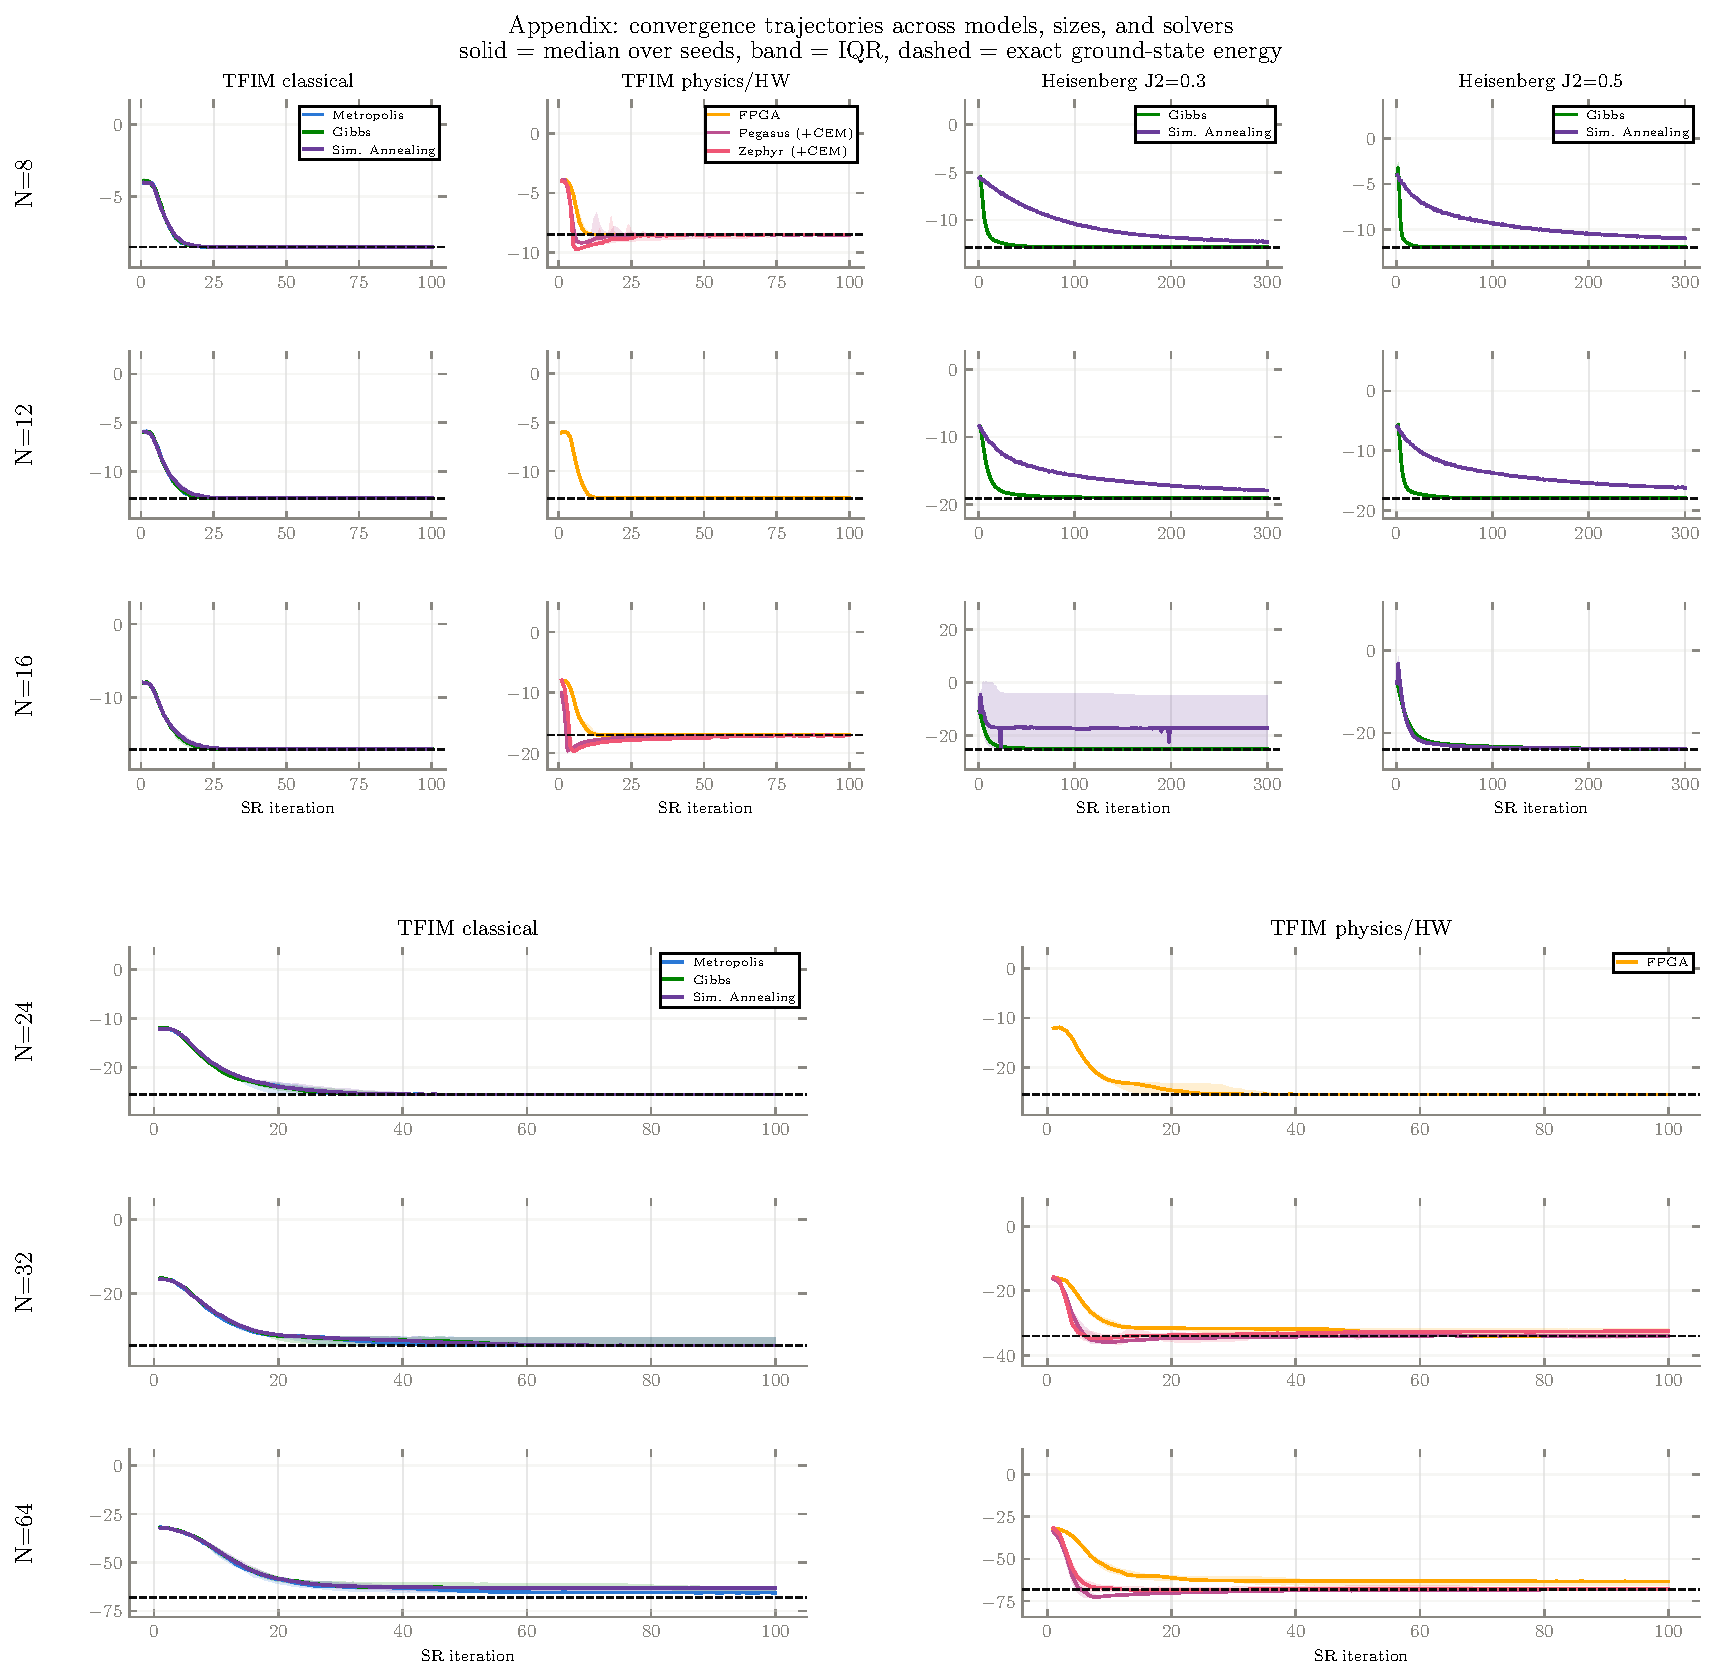
\includegraphics[width=\linewidth]{figures/fig12_appendix_size_solver_grid.pdf}
    \caption{Median per-iteration energy (IQR band) across system size $N$, physical model, and solver, dashed line marks the exact ground-state energy. Top block: $N=8,12,16$, all four columns. Bottom block: $N=24,32,64$, TFIM columns only (Heisenberg archive stops at $N=16$). TFIM columns use the \autoref{fig:tte_self_convergence} matched cell; Heisenberg columns use each cell's own per-instance-tuned hyperparameters (see text).}
    \label{fig:appendix_size_solver_grid}
\end{figure}
\clearpage
\bibliographystyle{unsrt}
\bibliography{bib}

\end{document}	
